%%%%%%%% ICML 2021 EXAMPLE LATEX SUBMISSION FILE %%%%%%%%%%%%%%%%%

\documentclass{article}

% Recommended, but optional, packages for figures and better typesetting:
\usepackage{microtype}
\usepackage{graphicx}
\usepackage{subfigure}
\usepackage{booktabs} % for professional tables

% hyperref makes hyperlinks in the resulting PDF.
% If your build breaks (sometimes temporarily if a hyperlink spans a page)
% please comment out the following usepackage line and replace
% \usepackage{icml2021} with \usepackage[nohyperref]{icml2021} above.


% Attempt to make hyperref and algorithmic work together better:
\newcommand{\theHalgorithm}{\arabic{algorithm}}

% Use the following line for the initial blind version submitted for review:
\usepackage{icml2021}
%!TEX root =  autocontgrlp.tex

\usepackage{multicol}
\usepackage{multirow}
\usepackage{dsfont}

%\setlength{\marginparwidth}{13mm}
\usepackage[textsize=tiny]{todonotes}
%\usepackage[disable]{todonotes}
\newcommand{\todoch}[2][]{\todo[color=blue!20!white,#1]{C: #2}}
%\usepackage{enumitem}
%\usepackage[fleqn]{amsmath}
\usepackage{amsmath}
\usepackage{hyperref}
\usepackage{cleveref}
\usepackage{mathtools}
\usepackage{graphicx}
\usepackage{times}
\usepackage{helvet}
\usepackage{courier}
\usepackage{paralist}
\usepackage{latexsym}
\usepackage{url}
\usepackage[all]{xy}
\usepackage{amsmath}
\usepackage{amssymb}
\usepackage{amsthm}
\usepackage{nccmath} % mfrac
\usepackage{comment}
%\usepackage{enumitem}
\usepackage{paralist}
\usepackage{xcolor}
%\usepackage[colorlinks=true,linkcolor=blue,citecolor=purple]{hyperref}
%\usepackage{hyperref}
\usepackage{graphicx}
\usepackage{pifont}
%\usepackage{algorithm}
%\usepackage{algorithmic}
%\usepackage{pseudocode}
%\usepackage{algpseudocode}
\usepackage{savesym}
\savesymbol{AND}
\usepackage{xspace}
\usepackage{tikz}
\usepackage{pgfplots}
\usepackage{pgf}
%\usepackage{algorithm}
%\usepackage{algorithmic}
\usepackage{xspace}
\usepackage{comment}
\usepackage{placeins}
%\usepackage[capitalize]{cleveref}
%\usepackage{caption}

%\usepackage{style/ssltr}
%\usepackage{style/macros}
\if0
\usetikzlibrary{intersections}
\usetikzlibrary{arrows,calc,fit,patterns,plotmarks,shapes.geometric,shapes.misc,shapes.symbols,   shapes.arrows,   shapes.callouts,   shapes.multipart,   shapes.gates.logic.US,   shapes.gates.logic.IEC,   er,   automata,   backgrounds,   chains,   topaths,   trees,   petri,   mindmap,   matrix,   calendar,   folding, fadings,   through,   positioning,   scopes,   decorations.fractals,   decorations.shapes,   decorations.text,   decorations.pathmorphing,   decorations.pathreplacing,   decorations.footprints,   decorations.markings, shadows,circuits}
\tikzstyle{decision}=[diamond,draw]
\tikzstyle{line}=[draw]
\tikzstyle{elli}=[draw,ellipse]
\tikzstyle{arrow} = [thick]
\fi
%\usepackage{subfig}

\newcommand{\rsa}{\rightsquigarrow}

\newcommand{\mb}{\mbox{ }}
\newcommand{\one}{\mathbf{1}}
\newcommand{\zero}{\mathbf{0}}
\newcommand{\nn}{\nonumber}


\newcommand{\R}{\Re} %{\mathbb{R}}
\newcommand{\Rm}{\mathbf{R}_{\min}}
\newcommand{\ra}{\rightarrow}
\newcommand{\om}{\otimes}
\newcommand{\op}{\oplus}
\newcommand{\RA}{\Rightarrow}
\newcommand{\LA}{\Leftarrow}
%\newcommand{\E}{\mathbb{E}}
\newcommand{\E}[1]{\mathbb{E}\left[#1\right]}
\newcommand{\lmin}[1]{\lambda_{\min}\left(#1\right)}
\newcommand{\T}{\mathcal{T}}
\newcommand{\B}{\mathcal{B}}
\newcommand{\F}{\mathcal{F}}
\newcommand{\C}{\mathcal{C}}
\newcommand{\M}{\mathcal{M}}
\newcommand{\N}{\mathcal{N}}

\newcommand{\I}{\mathcal{I}}

\newcommand{\mm}{m_{-}}
\newcommand{\mdm}{m'_{-}}
\newcommand{\Tvm}{\Theta^{v,\mm}}
\newcommand{\Tvmd}{\Theta^{v,\mdm}}


%\newcommand{\Tb}{\mathbf{\Theta}}
%\newcommand{\Tv}{\mathbf{\Theta}^v}
%\newcommand{\Tw}{\mathbf{\Theta}^w}
\newcommand{\tv}{\theta^v}

\newcommand{\Tb}{{\Theta}}
\newcommand{\Tv}{{\Theta}^v}
\newcommand{\Tw}{{\Theta}^w}
\newcommand{\Tg}{{\Theta}^g}

\newcommand{\tg}{\theta^g}
%\newcommand{\Tg}{\mathbf{\Theta}^g}
\newcommand{\Tt}{\Theta}

\newcommand{\G}{\mathcal{G}}

\DeclareMathOperator{\argmin}{argmin}
\DeclareMathOperator{\argmax}{argmax}
\newcommand{\norm}[1]{\|#1\|}
\newcommand{\inorm}[1]{\|#1\|_{\infty}}
\newcommand{\snorm}[1]{\left\|#1\right\|}
\newcommand{\sinorm}[1]{\left\|#1\right\|_{\infty}}


%\newcommand{\eqdef}{\stackrel{\text{\footnotesize def}}{=}}
%\newcommand{\eqdef}{\stackrel{\Delta}{=}}
\newcommand{\eqdef}{\doteq}
\newcommand{\defeq}{\doteq}

\newcommand{\eps}{\varepsilon}
\renewcommand{\epsilon}{\varepsilon}

\newcommand{\nt}{\nabla_{\Theta}}
\newcommand{\al}{\mathcal{AL}}
\newcommand{\aw}{\mathcal{AW}}
\newcommand{\ap}{\mathcal{AP}}

\newcommand{\keywords}[1]{{\bf Keywords: } #1\par}
%\newenvironment{proof}{{\bf Proof:} }{}
\newtheorem{theorem}{Theorem}[section]
\newtheorem{lemma}[theorem]{Lemma}
\newtheorem{claim}[theorem]{Claim}
\newtheorem{proposition}[theorem]{Proposition}
\newtheorem{corollary}[theorem]{Corollary}
\newtheorem{assumption}{Assumption}
\newtheorem{definition}{Definition}[section]
\newtheorem{remark}{Remark}[section]
\newtheorem{identity}{Identity}[section]
\newtheorem{example}{Example}[section]
\newtheorem{note}{Note}[section]
\newtheorem{notation}{Notation}[section]
\newcommand{\alert}[1]{\textcolor{red}{#1}} 
\newcommand{\J}{\mathcal{J}}
\newcommand{\ip}[1]{\langle #1\rangle}

\def\v{\mathbf{v}}
\def\r{\mathbf{r}}
\def\p{\mathbf{p}}
\def\q{\mathbf{q}}
%\def\R{\mathrm{R}}
\def\Re{\mathbb{R}}
\def\Z{\mathbb{Z}}
\def\P{\mathcal{P}}
\def\S{\mathcal{S}}
\def\A{\mathcal{A}}
\def\X{\mathcal{X}}
\def\U{\mathcal{U}}

%\newcommand{\B}{\mathcal{B}}


\newcommand{\ith}[2][th]{$#2^{\text{#1}}$}
\newcommand{\us}[2]{\underset{#2}{#1}~}
\newcounter{subequation}[equation]
\newcommand{\thesubequationonly}{\alph{subequation}}
\renewcommand{\thesubequation}{\text{\theequation(\thesubequationonly)}}
\newcommand{\subequationitem}{\refstepcounter{subequation}(\thesubequationonly)\thinspace}

\def\mathdisplay#1{%
  \ifmmode \@badmath
  \else
    $\def\@currenvir{#1}%
    \let\dspbrk@context\z@
    \let\tag\tag@in@display \SK@equationtrue %\let\label\label@in@display
    \global\let\df@label\@empty \global\let\df@tag\@empty
    \global\tag@false
    \let\mathdisplay@push\mathdisplay@@push
    \let\mathdisplay@pop\mathdisplay@@pop
    \if@fleqn
      \edef\restore@hfuzz{\hfuzz\the\hfuzz\relax}%
      \hfuzz\maxdimen
      \setbox\z@\hbox to\displaywidth\bgroup
        \let\split@warning\relax \restore@hfuzz
        \everymath\@emptytoks \m@th $\displaystyle
    \fi
%   \fi
}


% If accepted, instead use the following line for the camera-ready submission:
%\usepackage[accepted]{icml2021}```

% The \icmltitle you define below is probably too long as a header.
% Therefore, a short form for the running title is supplied here:
\icmltitlerunning{Submission and Formatting Instructions for ICML 2021}

\begin{document}

\twocolumn[
\icmltitle{Neural Tangent Kernel + Duality: From Alchemy To Atoms}

% It is OKAY to include author information, even for blind
% submissions: the style file will automatically remove it for you
% unless you've provided the [accepted] option to the icml2021
% package.

% List of affiliations: The first argument should be a (short)
% identifier you will use later to specify author affiliations
% Academic affiliations should list Department, University, City, Region, Country
% Industry affiliations should list Company, City, Region, Country

% You can specify symbols, otherwise they are numbered in order.
% Ideally, you should not use this facility. Affiliations will be numbered
% in order of appearance and this is the preferred way.
\icmlsetsymbol{equal}{*}

\begin{icmlauthorlist}
\icmlauthor{Chandrashekar}{}
\end{icmlauthorlist}

\icmlaffiliation{to}{Department of Computation, University of Torontoland, Torontoland, Canada}
\icmlaffiliation{goo}{Googol ShallowMind, New London, Michigan, USA}
\icmlaffiliation{ed}{School of Computation, University of Edenborrow, Edenborrow, United Kingdom}

\icmlcorrespondingauthor{Cieua Vvvvv}{c.vvvvv@googol.com}
\icmlcorrespondingauthor{Eee Pppp}{ep@eden.co.uk}

% You may provide any keywords that you
% find helpful for describing your paper; these are used to populate
% the "keywords" metadata in the PDF but will not be shown in the document
\icmlkeywords{Machine Learning, ICML}

\vskip 0.3in
]

% this must go after the closing bracket ] following \twocolumn[ ...

% This command actually creates the footnote in the first column
% listing the affiliations and the copyright notice.
% The command takes one argument, which is text to display at the start of the footnote.
% The \icmlEqualContribution command is standard text for equal contribution.
% Remove it (just {}) if you do not need this facility.

%\printAffiliationsAndNotice{}  % leave blank if no need to mention equal contribution
\printAffiliationsAndNotice{\icmlEqualContribution} % otherwise use the standard text.

\begin{abstract}
\emph{Is deep learning alchemy?} is a question that being currently debated. More than anything else, the lack of a \emph{pedagogical nugget} of ``simple experiments, simple theorems" is of concern. In this paper, we consider DNNs with rectified linear units (ReLUs). For such DNNs, we argue that two recent works namely (i) \emph{neural tangent kernel} and (ii) \emph{dual view}, combined together provide a useful pedagogical nugget.  In particular, we use dual view  to decompose the NTK into \emph{atomic} units in a manner that explains the role of weights, activations, width and depth unknown in prior literature.  We show that (i) weights: primary role of weights is to trigger the ReLU \emph{on/off} (i.e., $1/0$),  (ii) activations: each ReLU is a gate which provides a binary feature, (iii) width: stacking ReLUs widthwise in a layer gives rise to a base kernel which measures the \emph{average} number of triggered ReLUs, (iv) depth: stacking layers depthwise gives rise to a \emph{Hadamard product} 
%Finest atom is a ReLU, which is acts as a gate that blocks or passes its pre-activation input. Each gate is related to the hyperplane of the incoming weights, the gates in a layer give rise to a binary feature whose Gram matrix gives rise to the 
Our analysis shows that the standard view of features being learnt in the hidden layer outputs is a red-herring, and actual feature learning happens in the gates. Our paper builds on recent work which showed that the neural tangent kernel simplifies into a neural path kernel which encodes the information in the gates.
\end{abstract}

\section{Introduction}\label{sec:intro}
\subsection{Problem: Understanding Deep Neural Networks}
An important question plaguing machine learning \cite{BenAli-1,Lecun,BenAli-2,Aliresponse,Mickens} is:
\begin{center}
\textbf{\emph{Is Deep Learning Alchemy?}}
\end{center}
The \emph{alchemy} question can further be broken down into sub-questions/issues/gaps as listed below. 

1. \emph{Training:} Despite a \emph{non-convex} loss surface, why is it possible for stochastic gradient descent (SGD) (and its variants) to achieve zero training error in standard deep neural networks (DNNs)?

2. \emph{Generalisation:} Standard DNNs are \emph{over-parameterised}, yet, when trained on data with true labels we observe good test performance. Does understanding deep learning require rethinking generalisation? \cite{ben}

3. \emph{Depth:} Approximation results show that more depth is better \cite{depth1,depth2}, i.e., deeper models can approximate more complicated target functions better than shallow models. Yet, when training on standard datasets, increasing the depth beyond a point adversely affects both training and test performance \cite{resnets}. This situation can be remedied by using \emph{skip connections} giving rise to residual neural networks. However, why increasing depth beyond a point hurts standard DNNs is still not understood satisfactorily. 

4. \emph{Depth vs Width:} Wider models \cite{wide1,wide2,wide3} have also been quite successful. While increasing either depth or width causes an increase in the number of model parameters, the trade-off between width and depth is not clearly understood.

5. \emph{Functionality:} The roles of the basic parts namely weights and activation have not been clearly understood.

6. \emph{Uninterpretablity of Learnt Representation:} The commonly held view of feature learning is that lower level features are learnt in the initial layers and as one proceeds in depth more sophisticated features are learnt in the higher levels and the final layer learns a linear model in the features given by the output of the penultimate layer. However, there is no straightforward way to interpret the features learnt in the hidden layers.

7. There is a gap between \emph{universal approximation results} which characterise the class of functions representable by DNNs and \emph{practical} DNNs that are trained using SGD (and variants) starting from randomly initialised weights. Further, the performance of DNNs are evaluated on standard datasets such as MNIST and CIFAR-10. 

\subsection{Prior Work}
\subsubsection{Neural Tanget Kernel}
\begin{comment}{
As the alchemy question is being debated  \cite{BenAli-1,Lecun,BenAli-2,Aliresponse,Mickens} in the machine learning community, side by side theoretical as well as empirical efforts are begin made to obtain useful insights to understand DNNs. Common recurring themes in such works are (i) \emph{simplification} procedures such as pruning which involves systemically throwing away unnecessary weights and (ii) \emph{extremisation} approaches such as studying the behaviour of DNNs say in the limit of infinite width or say in the presence of random labels. Many a times such simplification/extremisation has resulted in more intriguing results and thrown further open questions. We will now describe some of these.

\textbf{Pruning} techniques have been known to reduce  the size of DNNs upto even $90\%$ without significant loss in performance \cite{prune1,prune2,prune3,prune4}. \cite{lottery} made an interesting observation that smaller networks pruned network can be re-trained to match the performance of the original unpruned network only when the pruned network is trained starting from its original initialisation. This lead to the so called \emph{lottery ticket} hypothesis, i.e., ``a randomly initialised, dense neural network contains a sub network that is initialised such that—when trained in isolation—it can match the test accuracy of the original network after training for at most the same number of iterations".

\textbf{Random Labels:} Training with random labels has been an extremisation approach. \cite{ben} showed that standard DNNs can achieve zero training error even when fitting random/shuffled labels, shuffled/random pixels on standard datasets. However, when trained on data with true uncorrupted labels, they achieve good test performance. In a recent paper, \cite{randlabel} showed pre-training with random labels could result in both \emph{positive} as well as \emph{negative} effect on the speed of downstream re-training with true labels depending on 	factors such as initialisation scale and number of random classes upstream. However, \cite{randlabel} also observe that the test performance of the downstream model always degrades when the model is pre-trained with random labels. It is an open question to understand this adverse effect on test performance.
}

{\textbf{Neural Tangent Kernel (NTK):} Recent works have shown that DNNs in the limit of infinite width are equivalent to kernel methods \cite{ntk,fcgp,convgp,arora2019exact,cao2019generalization}. Two important kernels associated with a (finite width) DNN are its \emph{conjugate kernel} derived from the output of the DNN and the so called \emph{neural tangent kernel} (NTK) based on the gradient of the output with respect to the DNN weights. As width approaches to infinity, both the conjugate and the neural tangent kernel converge to (their corresponding) deterministic matrices. It has been shown that training the last layer of the infinite width DNN is equivalent to a kernel method with the deterministic conjugate kernel and training  all the layers of an infinite width DNN is equivalent to a kernel method with the deterministic neural tangent kernel. Thus training and generalisation of infinite width DNNs boils down to the properties of the limiting deterministic kernel matrix. On a standard dataset such as CIFAR-10 the neural tangent kernel performs better than the conjugate kernel as well as other prior pure kernel based methods. However, standard finite width convolutional neural network still outperforms its infinite width neural tangent kernel counterpart by $5-6\%$. }
\end{comment}

Recent works have shown that DNNs in the limit of infinite width are equivalent to kernel methods \cite{ntk,fcgp,convgp,arora2019exact,cao2019generalization}. An important kernel associated with a (finite width) DNN is the so called \emph{neural tangent kernel} (NTK) based on the gradient of the output with respect to the DNN weights. As width approaches to infinity, both the neural tangent kernel converges to a limiting deterministic matrix. Hence, training and generalisation of infinite width DNNs boils down to the properties of the limiting deterministic kernel matrix. On a standard dataset such as CIFAR-10 the neural tangent kernel performs better than other prior pure kernel based methods. However, standard finite width convolutional neural network still outperforms its infinite width neural tangent kernel counterpart by $5-6\%$.

\textbf{Issues with NTK:} Even though the neural tangent kernel settles the training and generalisation questions in the case of infinite width DNNs, there are some interesting open questions. Firstly, we need to understand why  finite width neural networks outperform their infinite width neural tangent kernel counterparts. Secondly, it is not known why increasing the depth till a point makes the performance of the NTK also better.  %Thirdly, it is also not know why NTK corresponding to model with pooling performs better than models without pooling. Finally, feature learning is believed to be the unique differentiator of DNNs and other the machine learning methods, and neural tangent kernel being a kernel method has no feature learning.

\subsubsection{Duality and Neural Path Kernel}
Duality is of two kinds (a) \emph{network duality} and (b) \emph{weight duality}. Network duality says that DNNs with ReLU are both \emph{layers as well as paths}, and that the output of a DNN can be expressed as a summation of contribution of individual paths. For an input $x\in\R^{d_{\text{in}}}$, a path $p$'s contribution is equal $x(p)A_{\Theta}(p)v_{\Theta}(p)$, where $\Theta$ stands for network weights (i) $x(p)\in\R$ is the signal at the input node, (ii) $A_{\Theta}(p)$ is a binary feature which is $1$ if all the units in the path are \emph{triggered} and (iii) $v_{\Theta}(p)$ is the product of weights in the path. The weight duality is the observation that the weights $\Theta$ are responsible for both $A_{\Theta}$ and $v_{\Theta}$. 


We use dual view as a pedagogical nugget of ``simple theory and simple experiments'' \cite{Aliresponse} to obtain insights about `practical' deep neural networks (DNNs). The primal/dual view can be succinctly put as below. 
\begin{center}
\begin{tabular}{p{1cm}p{6cm}}
\emph{Primal:} & DNNs are composed of layers, and the output is obtained by proceeding layer by layer.\\
\emph{Dual:}& DNNs are composed of paths, and the output is obtained as a summation of path contributions.\\
\end{tabular}
\end{center}
 The dual view was exploited by \cite{npk} in the case of DNNs with ReLU activations. A special property of a ReLU is that it can also be seen as a gate/mask that blocks or allows its pre-activation input. 
{Using this gating property, the output of the DNN is expressed as summation of contribution of individual paths. Each path's contribution is equal to the product of the gates and weights in the path. The product gates are encodes in a neural path feature (NPF) and the product of weights are stored in a neural path value (NPV). }

\begin{center}
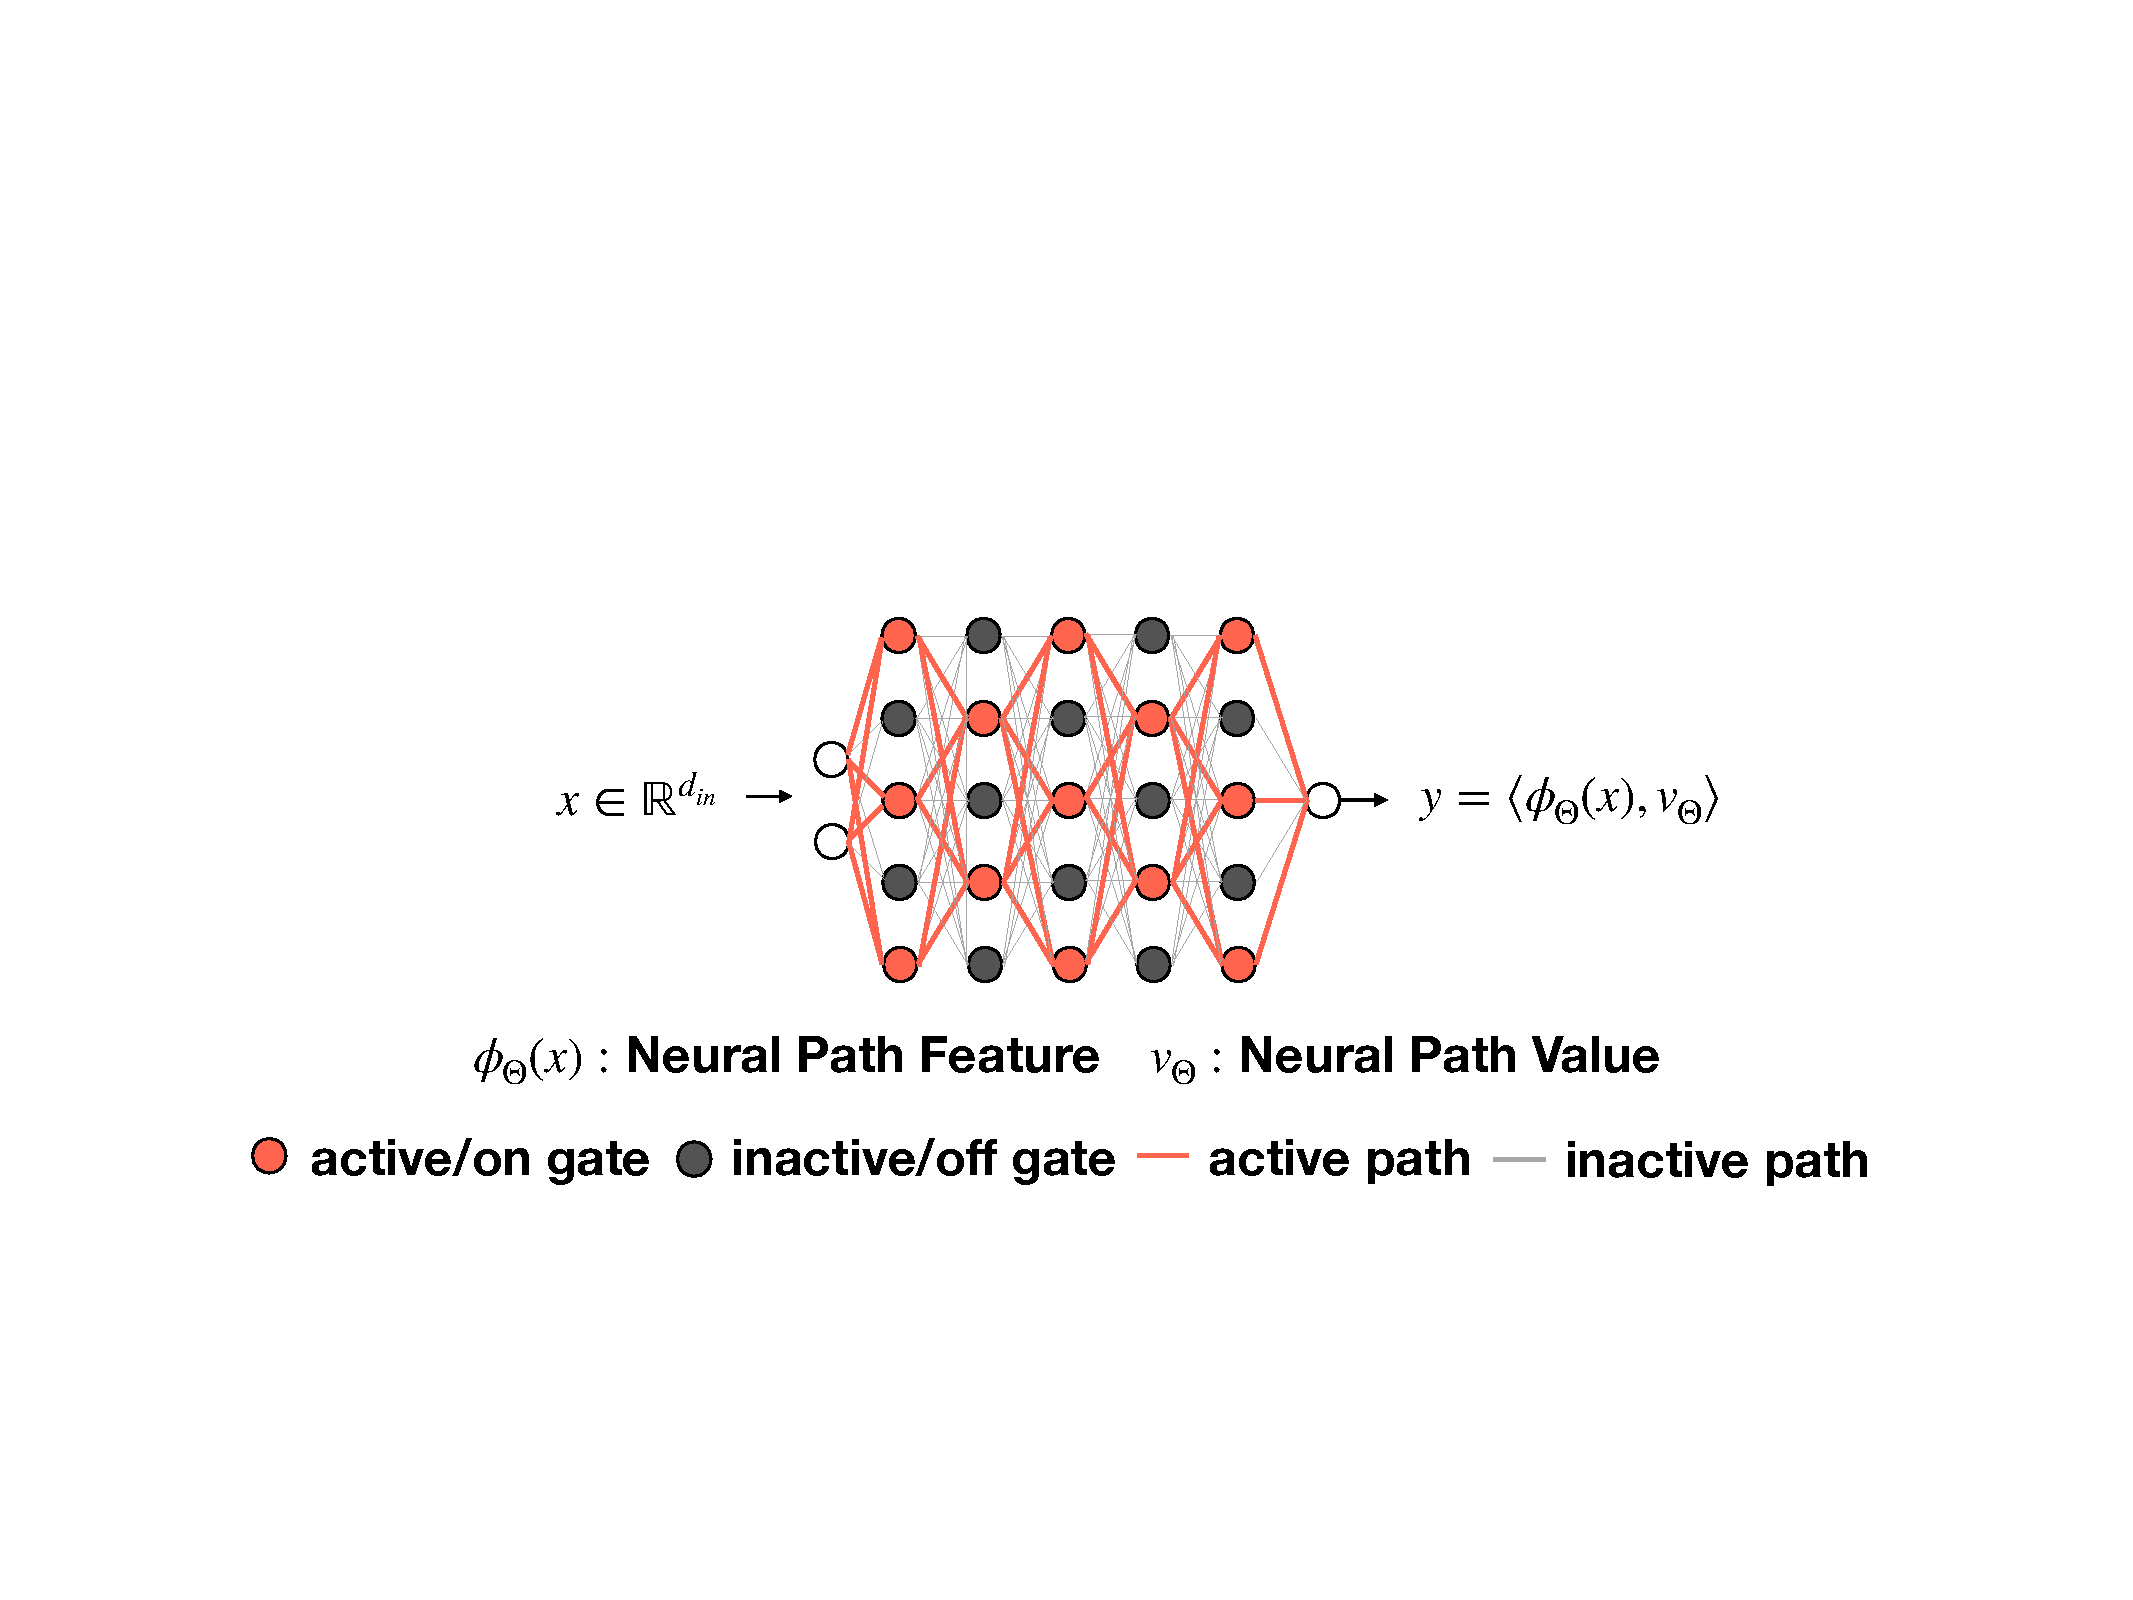
\includegraphics[scale=0.3]{figs/step1.pdf}
%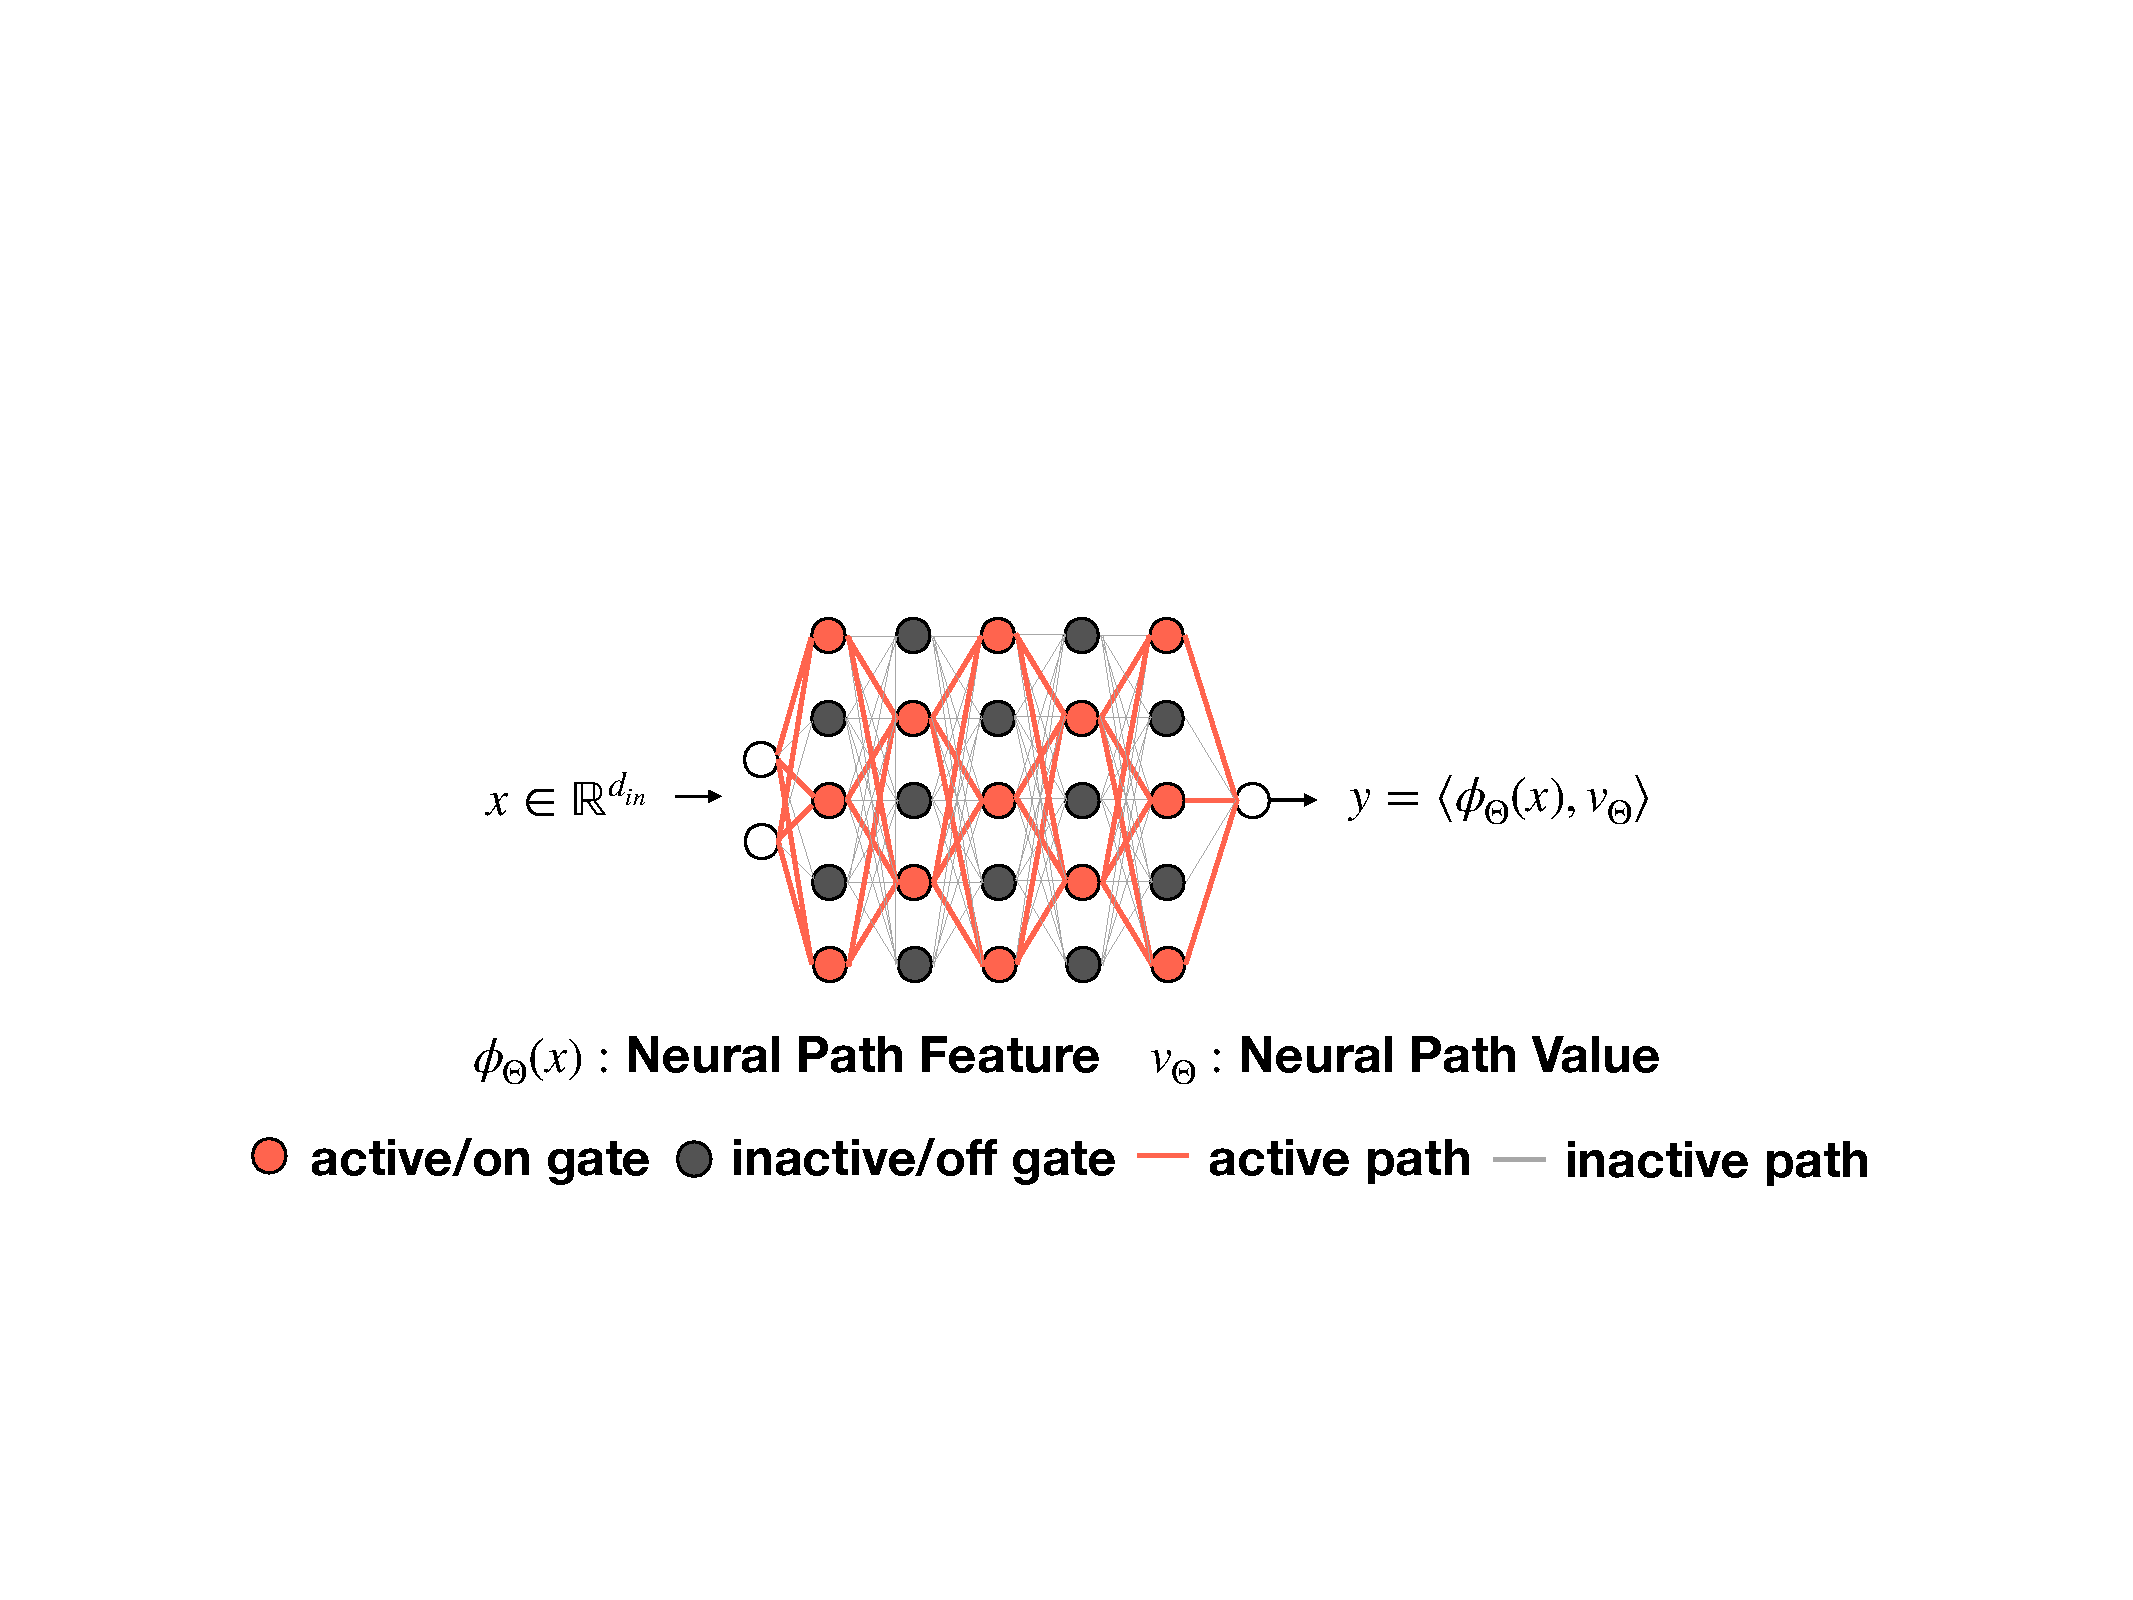
\includegraphics[scale=0.3]{figs/step1-center.pdf}
\end{center}


\begin{center}
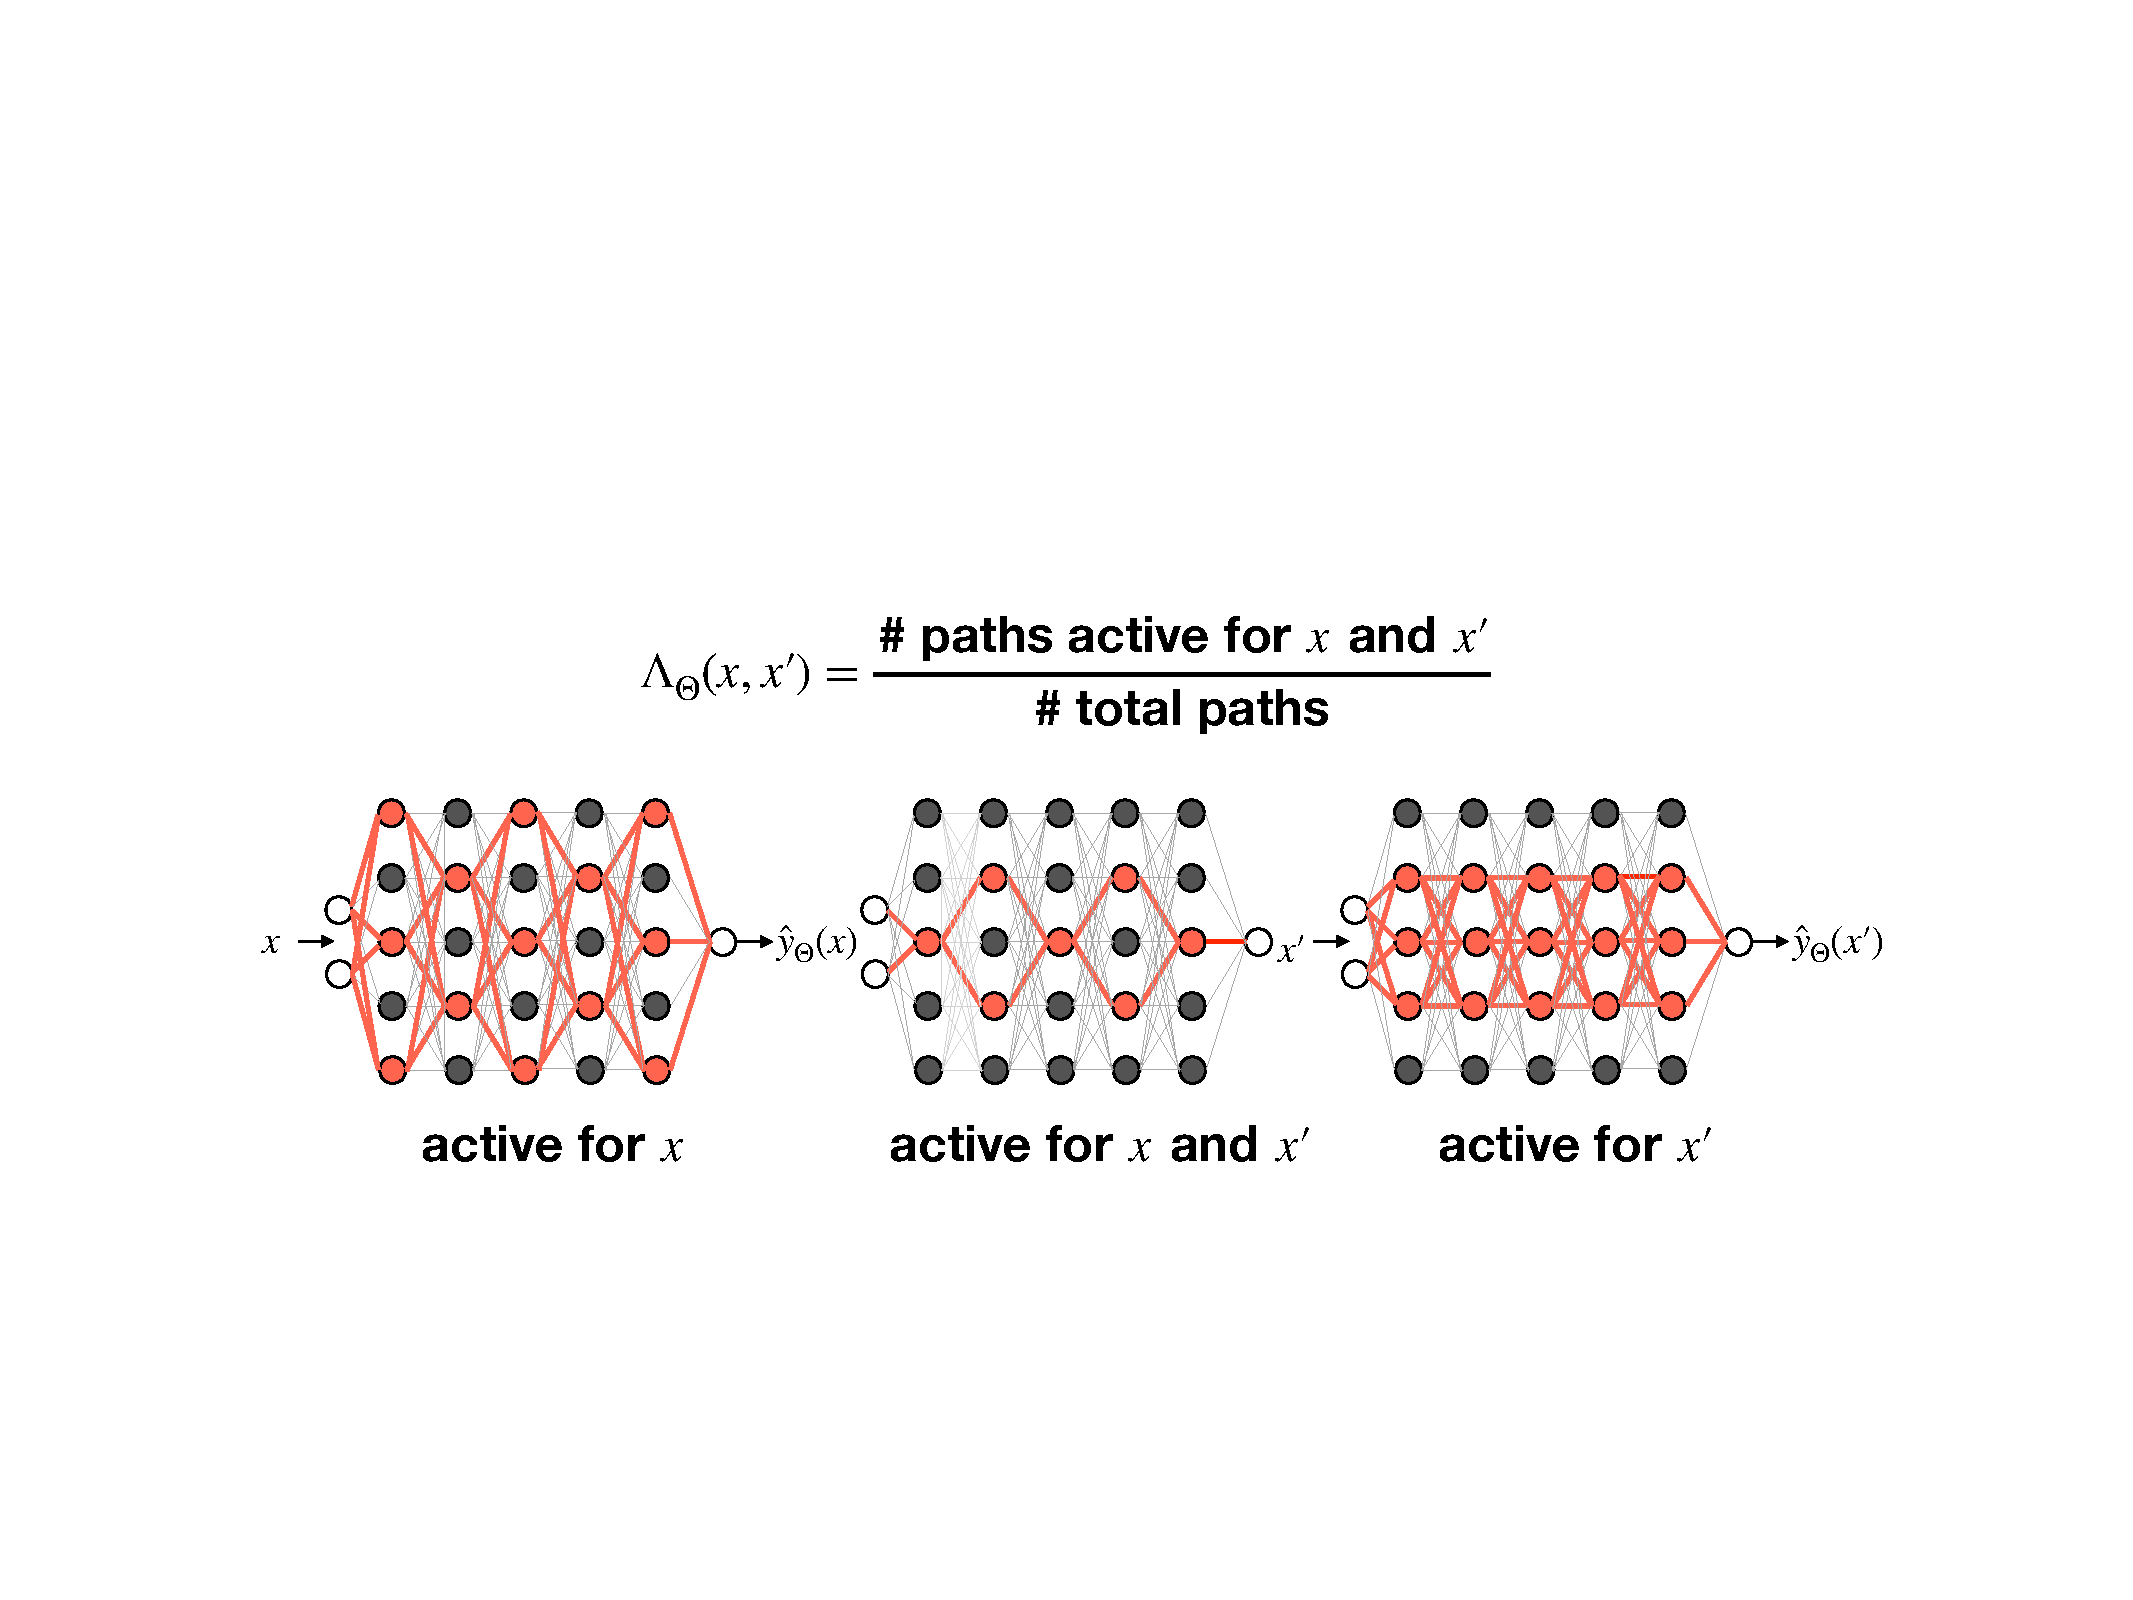
\includegraphics[scale=0.3]{figs/step2.pdf}
\end{center}


{By `practical', we mean DNNs with standard architectural choices (such as fully connected, convolutional, pooling layers, use of skip connections) trained using variants of stochastic gradient descent (SGD) starting from any of the widely used randomised initialisations. By `practical', we also mean to exclude theory that addresses solely approximation/capacity related questions \cite{depth1,depth2}.
}


\subsection{Our Contributions}



\begin{center}
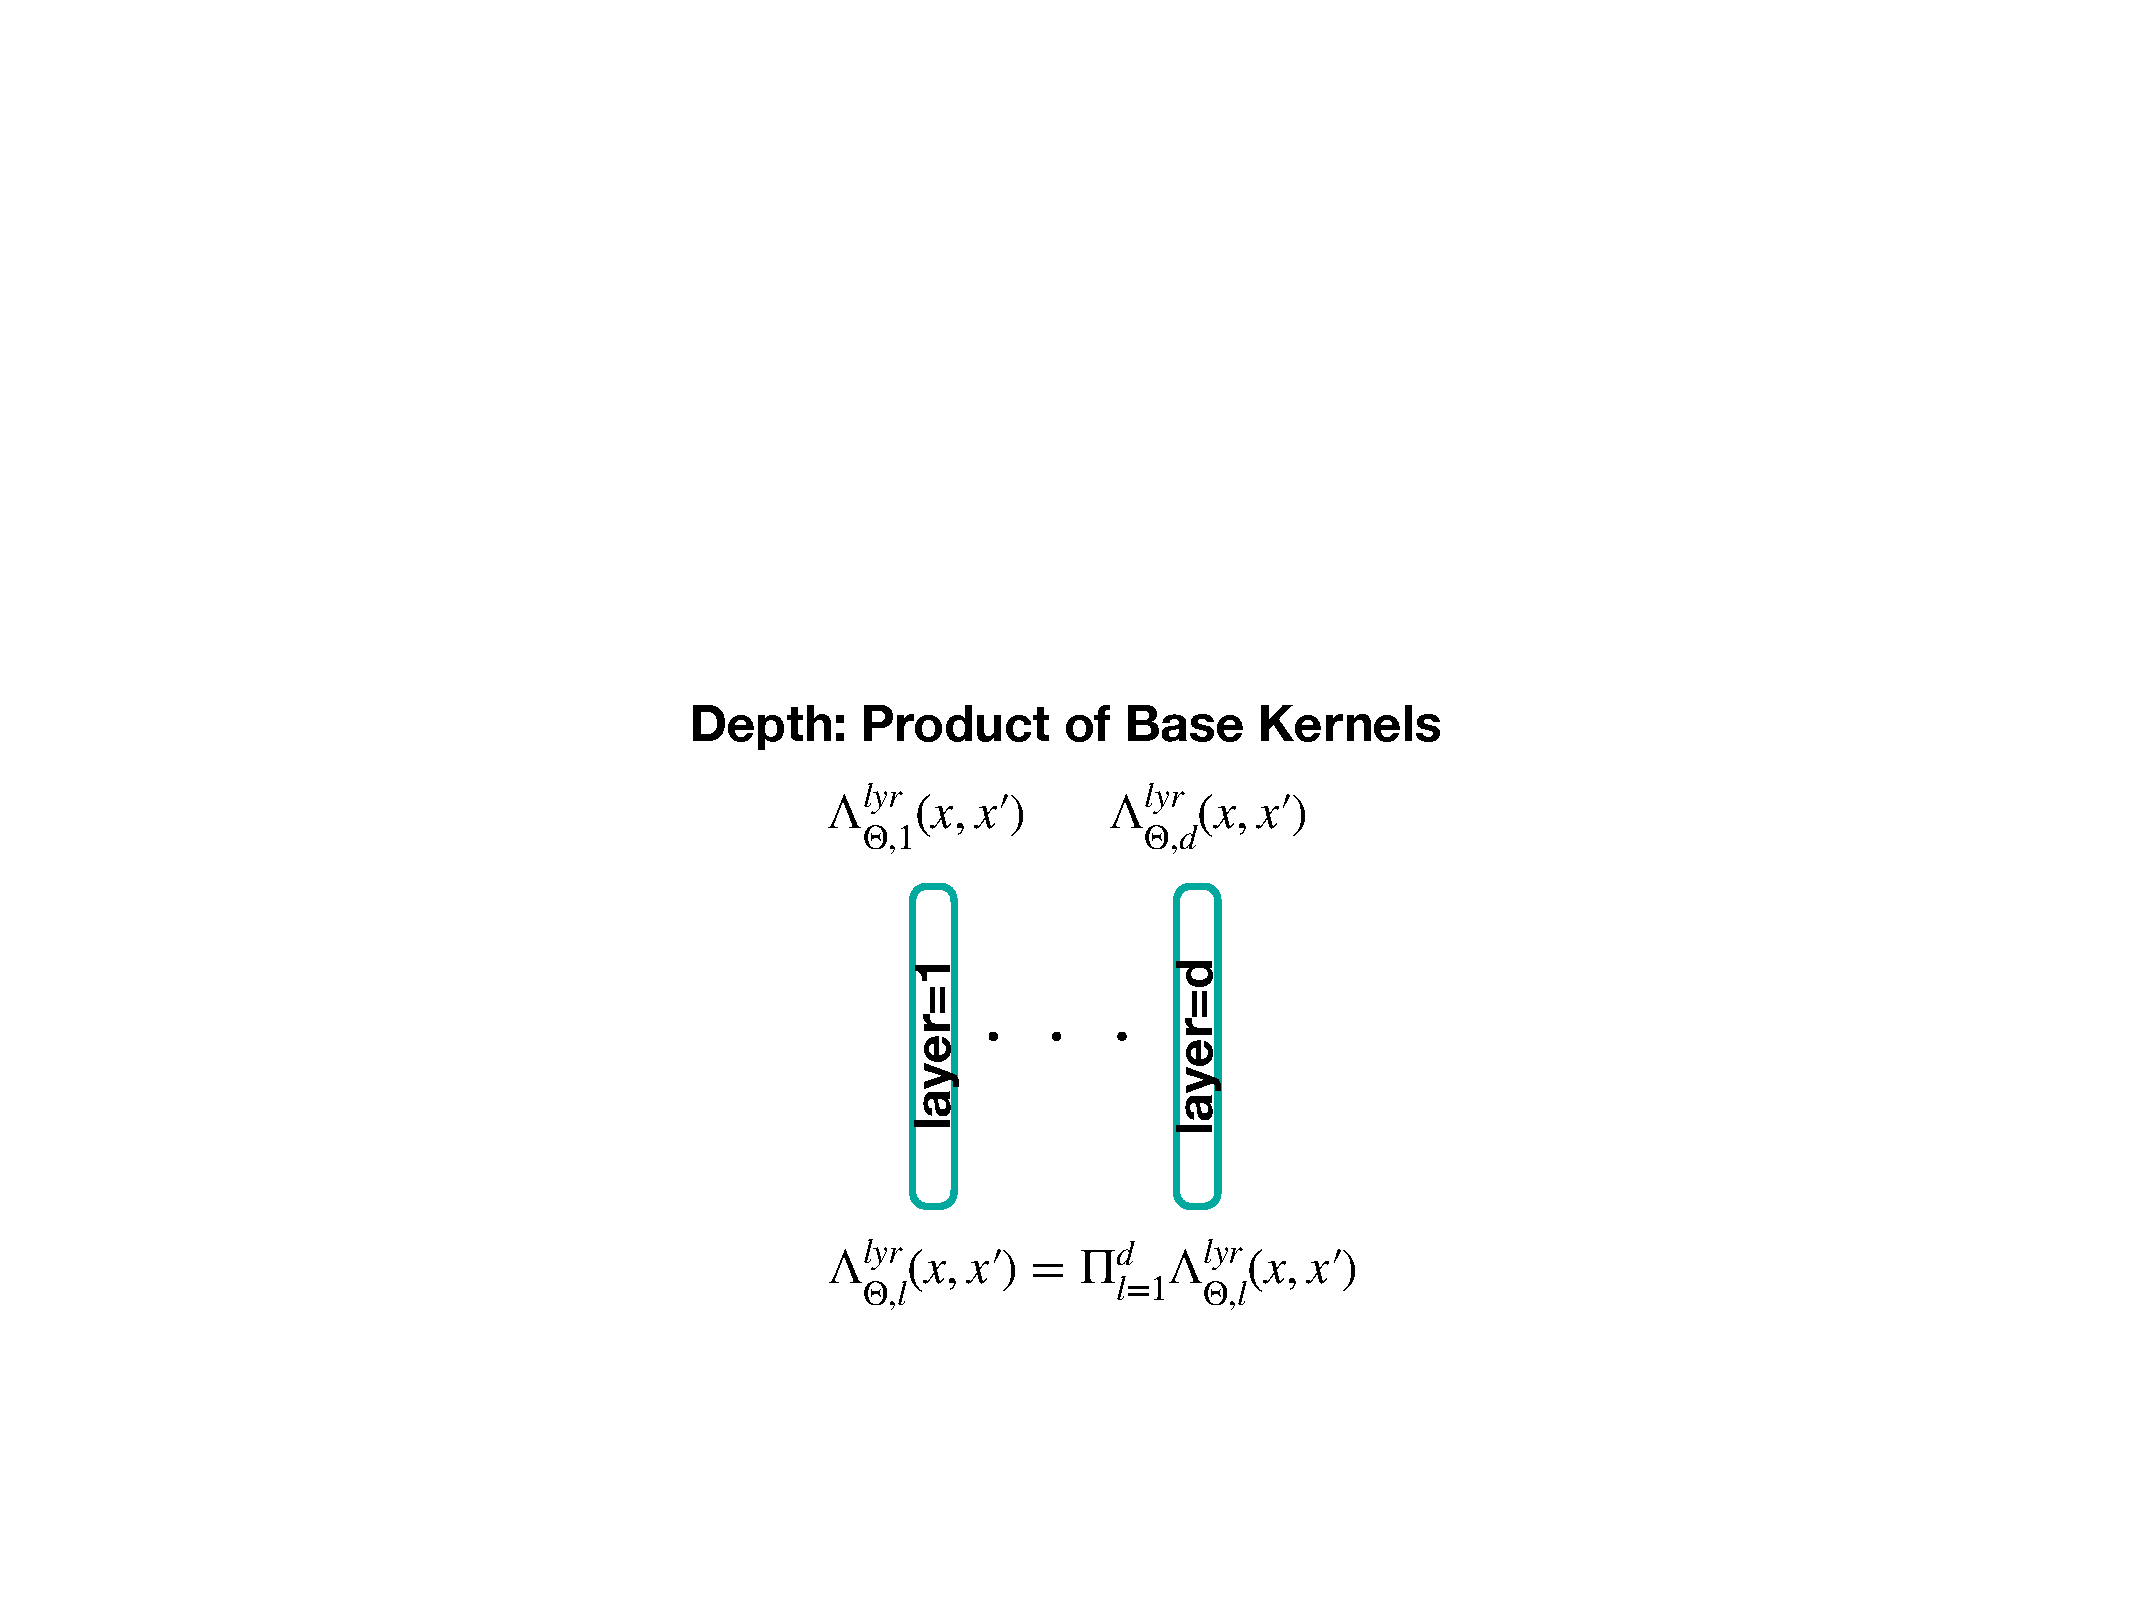
\includegraphics[scale=0.3]{figs/step4.pdf}
\end{center}

\begin{center}
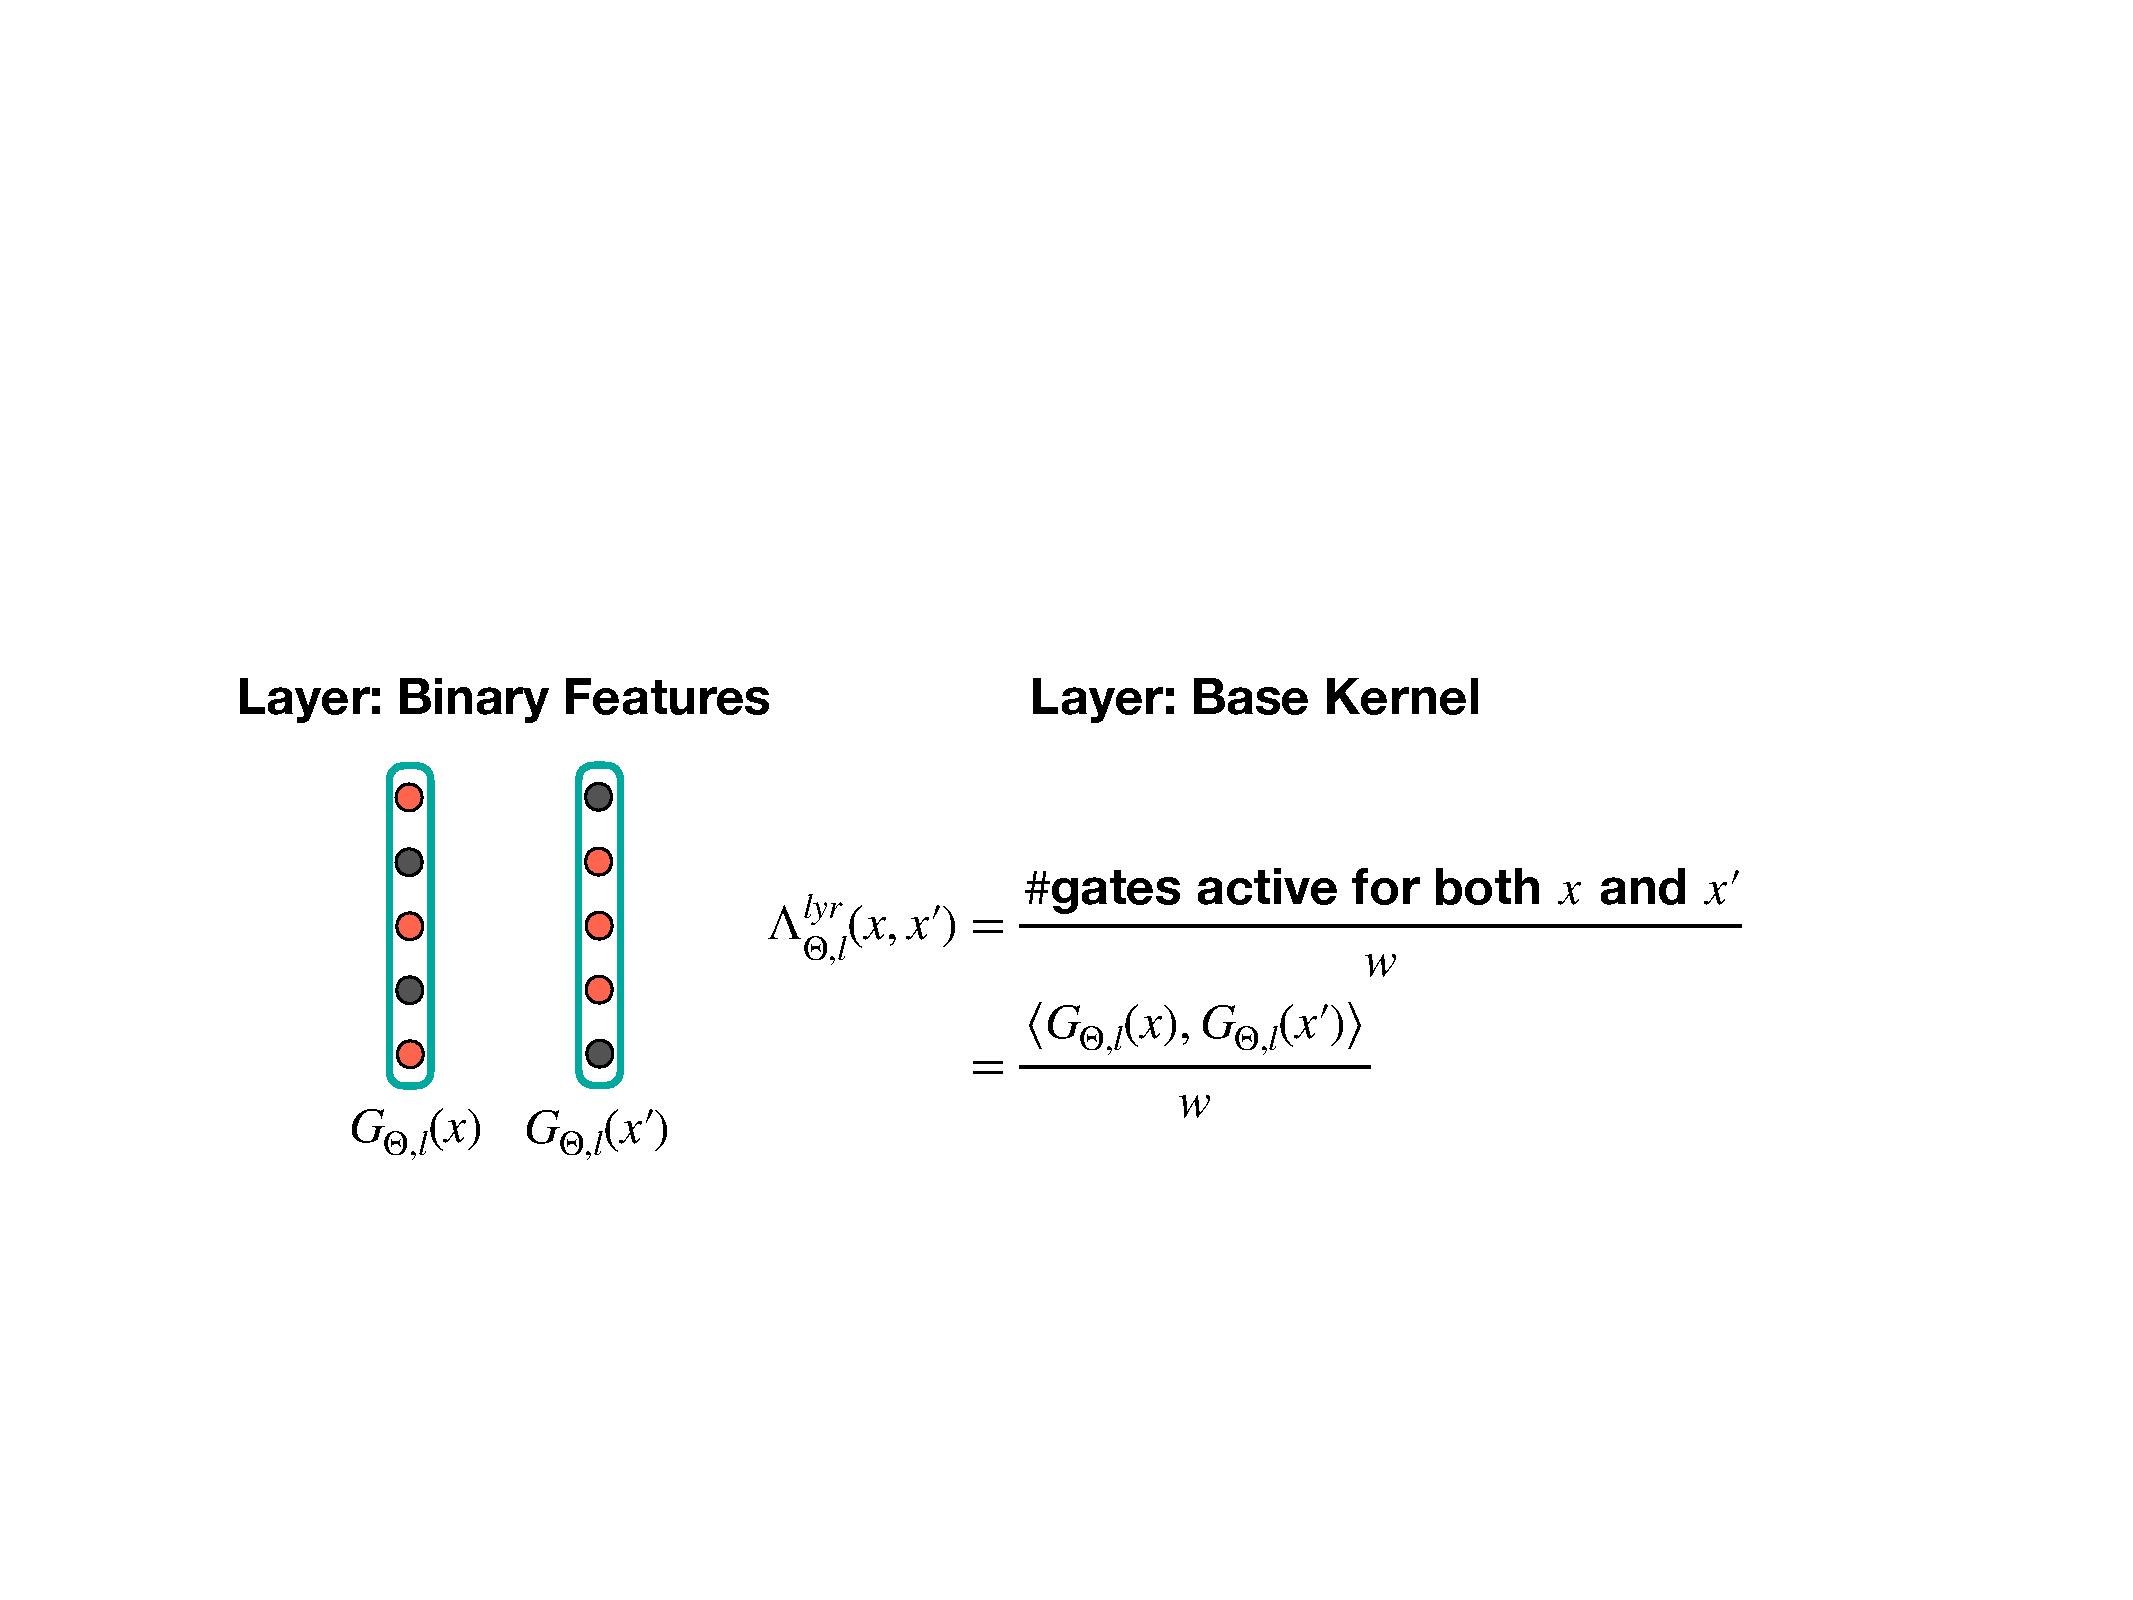
\includegraphics[scale=0.3]{figs/step3.pdf}
\end{center}


\subsection{Alchemy To Atoms:  Duality decomposes NTK }
\begin{center}
\textbf{\emph{Is Deep Learning Alchemy?}}
\end{center}
\begin{comment}
The neural tangent kernel (NTK) is defined using gradient of the DNN with respect to its weights, and it is known that training a randomly initialised infinite width DNN is equivalent to a kernel method with the NTK (i.e., infinite width limit of NTK) at initialisation. The dual view says that the DNN can broken down into paths, and output can be expressed as a summation of individual path contributions. Thus, the weights are responsible for both \emph{activating} a given path (by turning \emph{on} the ReLUs in the path) as well as \emph{amplifying} the signal at the input node of the path.
\end{comment}

\begin{comment}
\emph{Is deep learning alchemy?} The reason why this question is asked 
It is known that infinite width deep neural networks trained using gradient descent are equivalent to a kernel method using a fixed kernel matrix called the neural tangent kernel. A recent work has shown that in the case of DNNs with rectified linear units (ReLU), 
 The answer is \emph{no}. 
We look at deep neural networks (DNNs) with rectified linear unit (ReLU) activations. Recent works have connected, 
 which have two kinds of dualities (a) \emph{network duality} and (b) \emph{weight duality}. Network duality says that DNNs with ReLU are both \emph{layers as well as paths}, and that the output can be expressed as a summation of contribution of individual paths. The weight duality says that the weights are responsible for both \emph{activating} a given path (by turning \emph{on} the ReLUs in the path) as well as \emph{amplifying} the signal at the input node of the path.

We use \emph{duality} as a \emph{pedagogical nugget} to argue that deep learning is not \emph{alchemical} but can be \emph{atomised}, i.e., hierarchically broken down into of simpler units. At most basic level are the ReLUs which store the binary features (\emph{on/off}). Each layer corresponds to a \emph{base kernel} which measures the \emph{average} number of ReLUs `on' in that layer for a given pair input examples. While width gives averaging in the base kernel, depth gives rise to a \emph{product of base kernels}.


\end{comment}


\bibliographystyle{plainnat}
\bibliography{refs}
%%\section{Neural Path Framework For CNN}\label{sec:cnpf}
\textbf{Indexing:} The weights of layers $l\in[\dc]$ are denoted by $\Theta(\icin,\iin,\iout,l)$ and for layers $l\in[\dfc]+\dc$ are denoted by $\Theta(\iin,\iout,l)$. The pre-activations, gating and hidden unit outputs are denoted by $q_{x,\Theta}(\ifout,\iout,l)$,  $G_{x,\Theta}(\ifout,\iout,l)$, and $z_{x,\Theta}(\ifout,\iout,l)$ for layers $l=1,\ldots, \dc$. $\iin$ and $\iout$ are used to index the input and the output filters. $\ifout$ is used to denote the index of hidden unit (in the feature dimension) within the input and output filters. %Here, $\icin\in[\wconv]$, for $l=1\ldots,\dc$, $\iin\in[w]$ for $l=\dc+2,\ldots,\dc+\dfc+1$, $\ifin \in[1]$ for $l=1$, $\ifin \in[w]$ for $l=2,\ldots,\dc$, $\iout\in[w]$ for $l=1\ldots,\dc, \dc+2,\ldots, \dc+\dfc$,  $\iout\in[1]$ for $l=\dc+\dfc+1$, $\ifout\in[w]$ for $l=1,\ldots,\dc$.
\begin{comment}
\FloatBarrier
\begin{table}[h]
\centering
\begin{tabular}{|c|ll|}\hline
Index & Range&\\\hline
\multirow{2}{*}{$\iin$} & $\in[\din]$ & for $l=1\ldots,\dc$\\ \cline{2-3}
&$\in[w]$ & for $l=\dc+2,\ldots,\dc+\dfc+1$\\ \hline
\multirow{2}{*}{$\ifin$} & $\in[1]$ & for $l=1$\\ \cline{2-3}
&$\in[w]$ &for $l=2,\ldots,\dc$\\ \hline
\multirow{2}{*}{$\iout$} & $\in[w]$ &for $l=1\ldots,\dc, \dc+2,\ldots, \dc+\dfc$\\ \cline{2-3}
&$\in[1]$ &for $l=\dc+\dfc+1$\\ \hline
{$\ifout$} & $\in[w]$ &for $l=1,\ldots,\dc$\\ \hline
\end{tabular}
\end{table}
\end{comment}

\textbf{Shapes:} \Cref{fig:shape-main} shows the shapes of the tensors in the convolutional layers of a $1$-dimensional circular CNN considered in this paper. Here, the input is a $1$-dimensional tensor given by $x\in\R^{\din}$. The hidden nodes in a given convolutional layer have a $2$-dimensional shape of $\din\times w$, where $w$ is the number of filters in the layer. The weights of a given convolutional layer have $3$-dimensional shape of $\wconv\times w\times w$,  where $w\times w$ is because of the number of input filters times the number of output filters.
\FloatBarrier
\begin{figure}[h]
\centering
%\resizebox{\columnwidth}{!}{
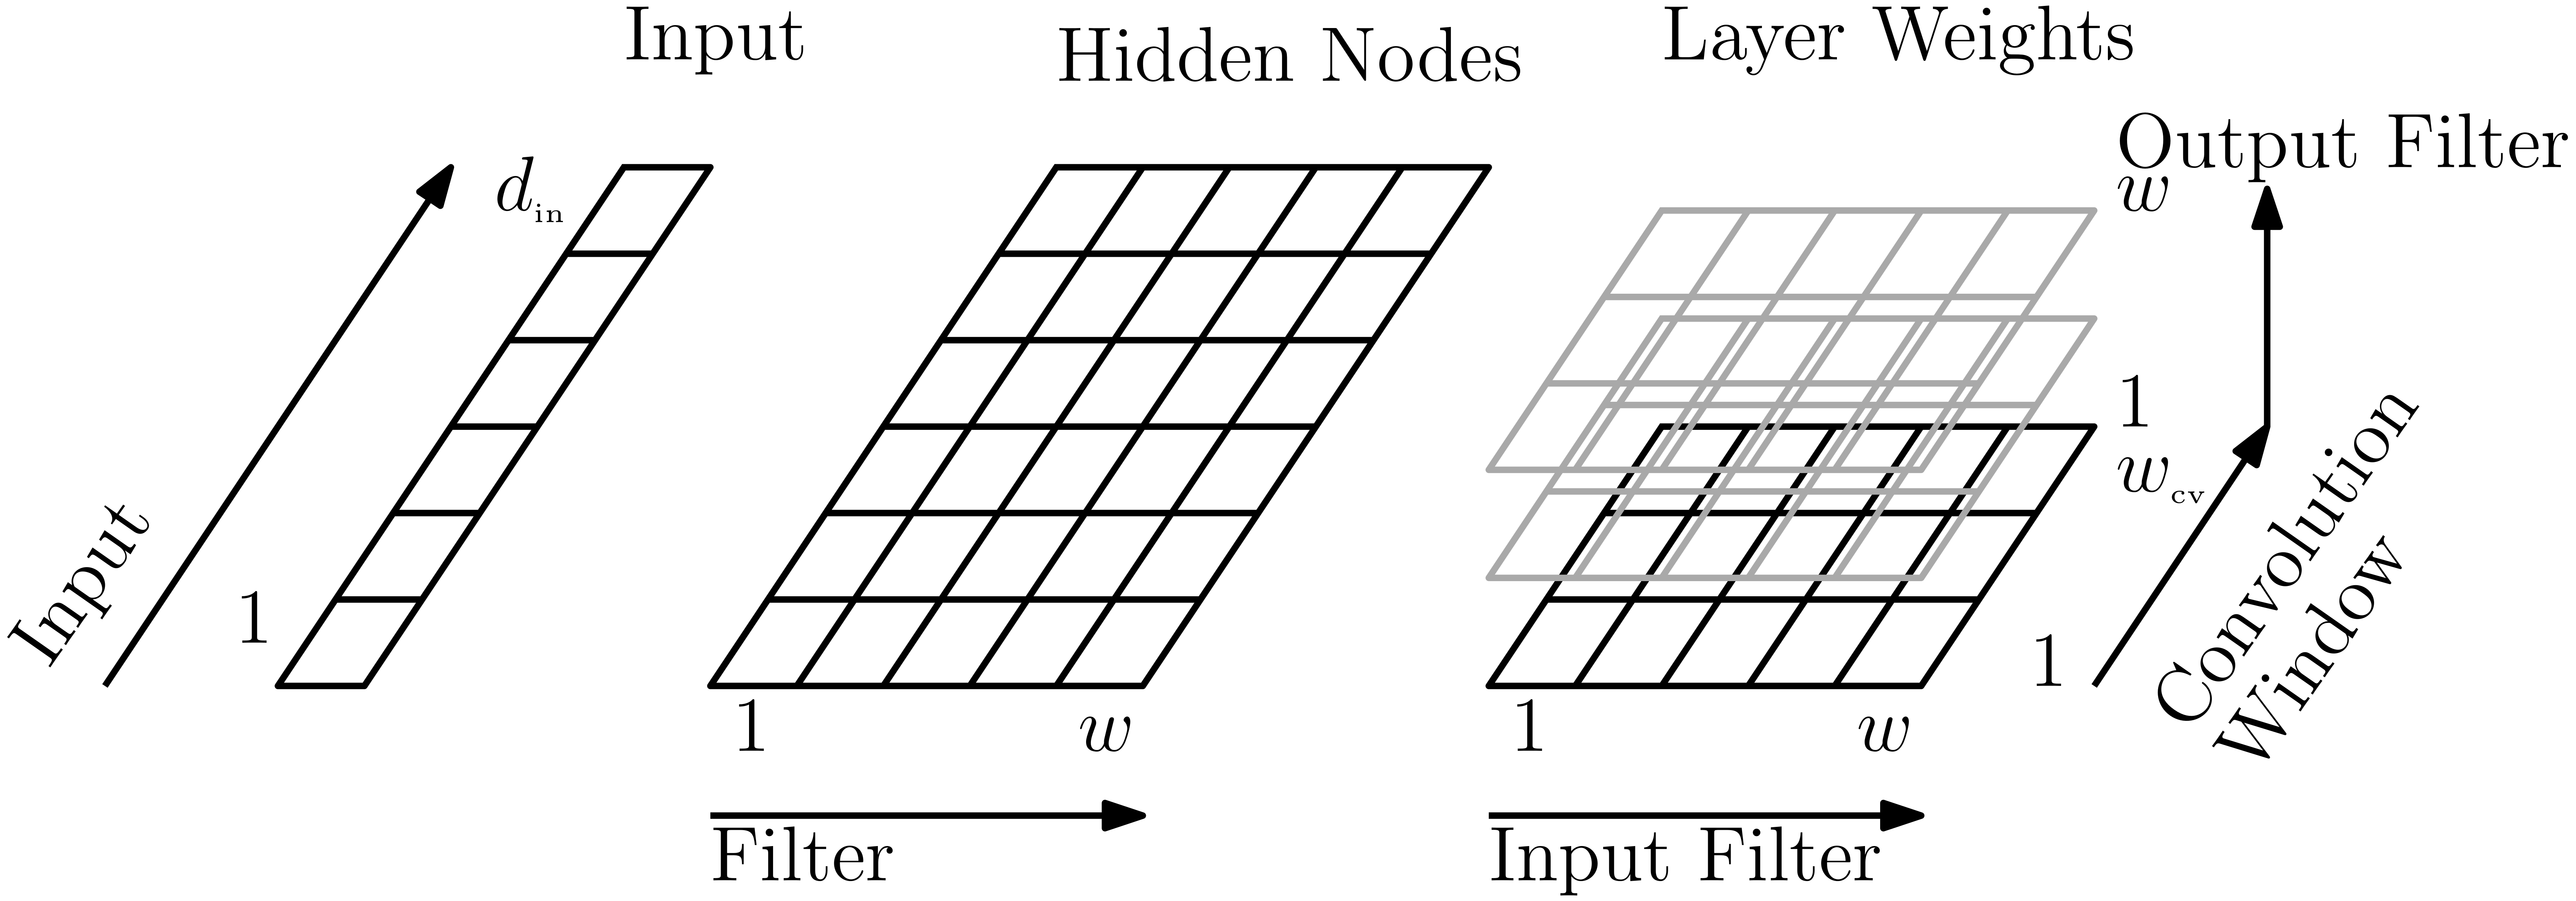
\includegraphics[scale=0.04]{figs/shape.png}
%}
\label{fig:shape-main}
\caption{Shows the shape of the tensor.}
\end{figure}

\subsubsection{Information Flow}
\begin{table}[h]
\centering
\begin{tabular}{|c l lll|}\hline
IL&: &$z_{x,\Theta}(\cdot,1,0)$ &$=$ &$x$ \\\hline\hline
\multicolumn{5}{|l|}{Convolutional Layers, $l\in[\dc]$}\\\hline\hline
PA&: & $q_{x,\Theta}(\ifout,\iout,l)$& $=$ & $\sum_{\icin,\iin}\Theta(\icin,\iin,\iout,l)\cdot z_{x,\Theta}(\ifout\oplus (\icin-1),\iin,l-1)$\\
GV&: &$G_{x,\Theta}(\ifout,\iout,l)$& $=$ & $\mathbf{1}_{\{q_{x,\Theta}(\ifout,\iout,l)>0\}}$\\
HUO&: &$z_{x,\Theta}(\ifout,\iout,l)$ & $=$ & $q_{x,\Theta}(\ifout,\iout,l)\cdot G_{x,\Theta}(\ifout,\iout,l)$\\\hline\hline
\multicolumn{5}{|l|}{GAP Layers, $l=\dc+1$}\\\hline\hline
%HUO&: &${z}_{x,\Theta}(\iout,l)$ & $=$ & $\frac{1}{\din}\sum_{i\in [\din]} z_{x,\Theta}(i,\iout,l-1)$\\\hline\hline
HUO&: &$z_{x,\Theta}(\iout, \dc+1)$ & $=$ &$\sum_{\ifout} z_{x,\Theta}(\ifout,\iout,\dc)\cdot G^{\text{pool}}_{x,\Theta}(\ifout,\iout,\dc+1)$\\\hline\hline
\multicolumn{5}{|l|}{Fully Connected Layers, $l\in[\dfc]+(\dc+1)$}\\\hline\hline
PA&: & $q_{x,\Theta}(\iout,l)$& $=$ & $\sum_{\iin}\Theta(\iin,\iout,l) \cdot z_{x,\Theta}(\iin,l-1) $\\
GV&: &$G_{x,\Theta}(\iout,l)$& $=$ & $\mathbf{1}_{\{(q_{x,\Theta}(\iout,l))>0\}}$\\
HUO&: &$z_{x,\Theta}(\iout,l)$ & $=$ & $q_{x,\Theta}(\iout,l)\cdot G_{x,\Theta}(\iout,l)$\\
FO&: & $\hat{y}_{\Theta}(x)$ & $=$ & $\sum_{\iin}\Theta(\iin,\iout, d)\cdot z_{x,\Theta}(\iin,d-1)$\\\hline
\end{tabular}
\caption{Here IL, PA, GV, HUO, GL and FO are abbreviations for input layer, pre-activation, gating values, hidden unit output, GAP-layer and final output respectively.}
\label{tb:cconv}
\end{table}

\FloatBarrier
\begin{figure}[H]
\centering
\resizebox{\columnwidth}{!}{
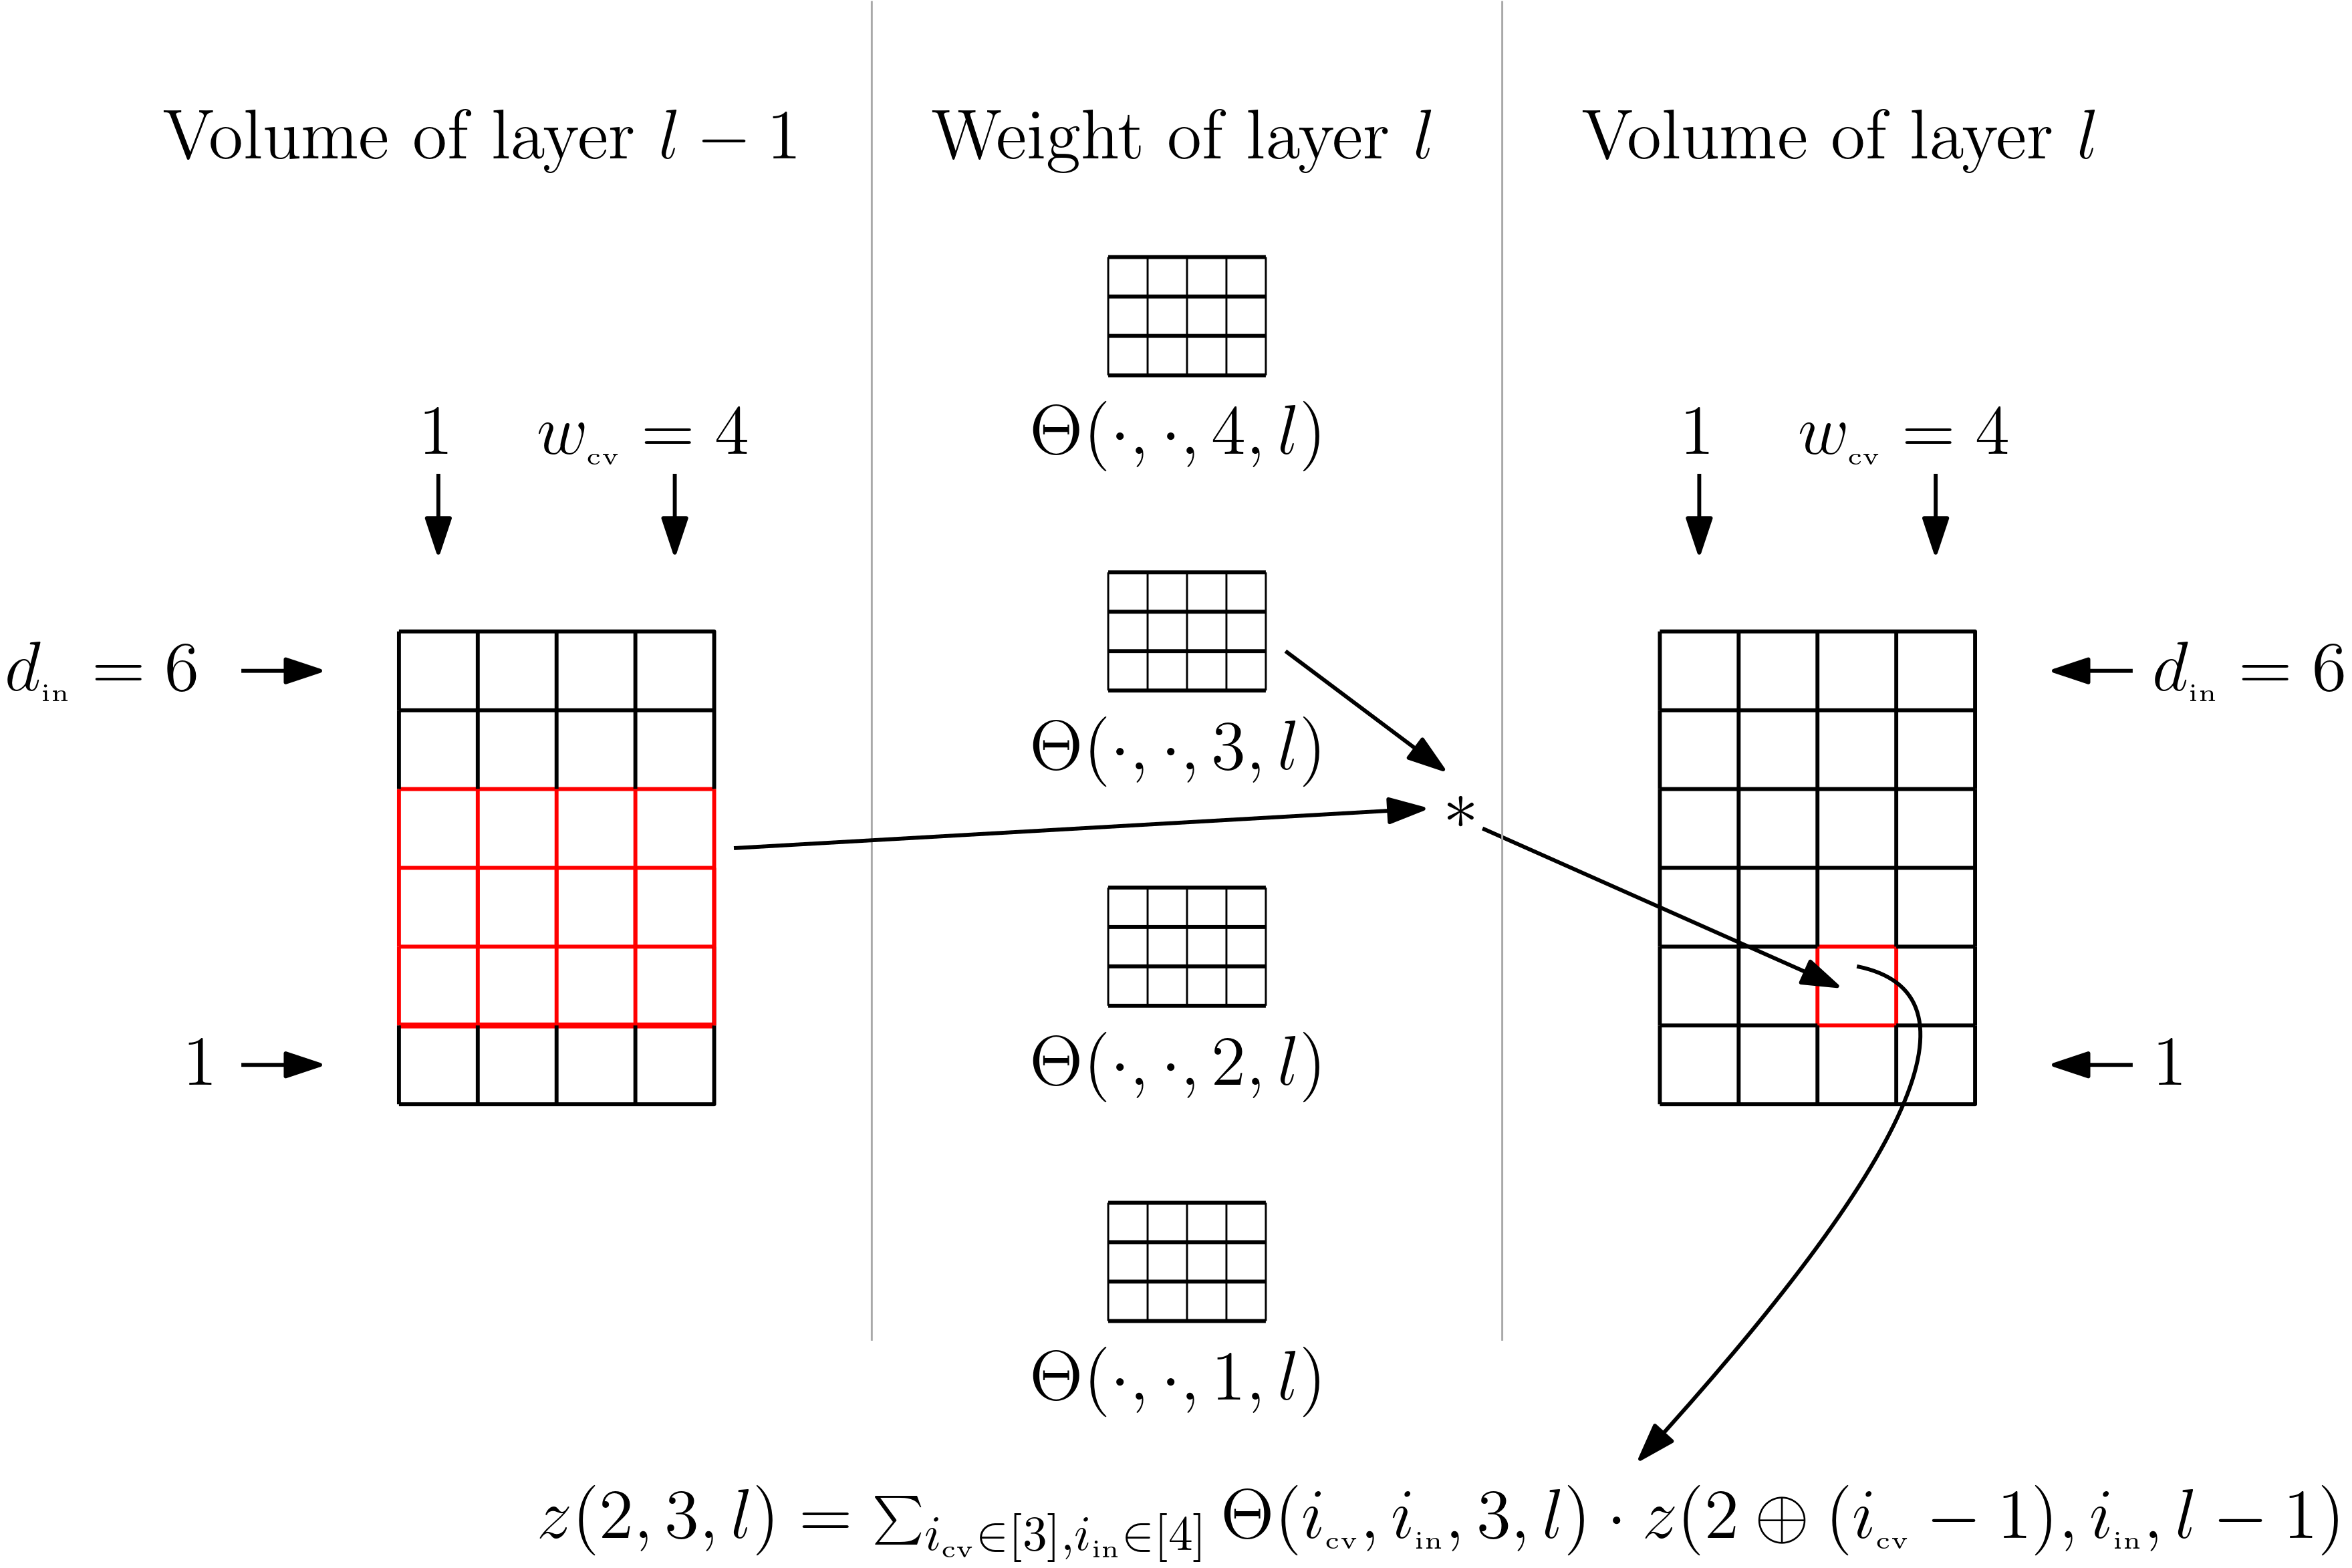
\includegraphics[scale=1]{figs/single-filter.png}
}
\end{figure}
\newpage

%%\input{supp}
%\newpage
\begin{center}
{\Large{\textbf{Appendix}}}
\end{center}

\begin{appendix}
\section{Expression for $K^{(d)}$}\label{sec:kd}
The $K^{(d)}$ matrix is computed by the recursion in \eqref{eq:ntkold}.
\begin{align}\label{eq:ntkold}
&\tilde{K}^{(1)}(s,s')=\Sigma^{(1)}(s,s')=\Sigma(s,s'), M^{(l)}_{ss'}=\left[\begin{matrix}\Sigma^{(l)}(s,s) & \Sigma^{(l)}(s,s')\\ \Sigma^{(l)}(s',s) & \Sigma^{(l)}(s',s')\end{matrix}\right]\in \R^2,\nn\\
&\Sigma^{(l+1)}(s,s')= 2\cdot\mathbb{E}_{(q,q')\sim N(0,M_{ss'}^{(l)})} \left[\chi(q)\chi(q')\right], \hat{\Sigma}^{(l+1)}(s,s')= 2\cdot\mathbb{E}_{(q,q')\sim N(0,M_{ss'}^{(l)})}\left[\partial\chi(q)\partial{\chi}(q')\right],\nn\\
&\tilde{K}^{(l+1)}=\tilde{K}^{(l)}\odot \hat{\Sigma}^{(l+1)}+\Sigma^{(l+1)}, K^{(d)}=\left(\tilde{K}^{(d)}+\Sigma^{(d)}\right)/2
\end{align}
where $s,s'\in[n]$ are two input examples in the dataset, $\Sigma$ is the data Gram matrix, $\partial{\chi}$ stands for the derivative of the activation function with respect to the pre-activation input, $N(0,M)$ stands for the mean-zero Gaussian distribution with co-variance matrix $M$.



\section{Proofs of technical results}
\textbf{Proof of \Cref{prop:basic}}
\begin{proof}
We know that $e_t=(e_t(s),s\in[n])\in\R^n$, and $e_t(s)=\hat{y}_{\Theta_t}(x_s)-y(s)$. Now
\begin{align} 
L_{\Theta_t}&=\frac{1}2\sum_{s'=1}^n(\hat{y}_{\Theta_t}-y)^2\nn\\
&=\frac{1}2\sum_{s'=1}^n e_t^2\nn\\
\nabla_{\Theta} L_{\Theta_t}&= \sum_{s'=1}^n\nabla_{\Theta} \hat{y}_{\Theta_t}(x_{s'})e_t(s')\nn\\
\label{eq:above1} \nabla_{\Theta} L_{\Theta_t}&= \sum_{s'=1}^n \psi_{x_{s'},\Theta_t}e_t(s')
\end{align}
For gradient descent, $\dot{\Theta}_t=-\nabla_{\Theta} L_{\Theta_t}$, from \eqref{eq:above1} it follows that 
\begin{align}
\dot{\Theta}_t=-\sum_{s'=1}^n \psi_{x_{s'},\Theta_t}e_t(s')
\end{align}
Now $\dot{e}_t=\dot{\hat{y}}_{\Theta_t}$, and expanding $\dot{\hat{y}}_{\Theta_t}(x_s)$ for some $s\in[n]$, we have:
\begin{align}
\dot{\hat{y}}_{\Theta_t}(x_s)&=\frac{d \hat{y}_{\Theta_t}(x_s)}{d t}\nn\\
&=\sum_{\theta\in\Theta}\frac{d \hat{y}_{\Theta_t}(x_s)}{d \theta}\frac{d \theta_t}{dt},\,\text{by expressing this summation as a dot product we obtain} \nn\\
\dot{\hat{y}}_{\Theta_t}(x_s)&=\ip{\psi_{x_s,\Theta_t},\dot{\Theta}_t}
\end{align}
We now use that fact that $\Theta_t$ is updated by gradient descent
\begin{align}
\dot{\hat{y}}_{\Theta_t}(x_s)&=-\ip{\psi_{x_s,\Theta_t},\sum_{s'=1}^n \psi_{x_{s'},\Theta_t}e_t(s')}\nn\\
&=-\sum_{s'=1}^n K_{\Theta_t}(s,s')e_t(s')
\end{align}
The proof is complete by recalling that $\hat{y}_{\Theta_t}=(\hat{y}_{\Theta_t}(x_s),s\in[n])$, and $\dot{e}_t=\dot{\hat{y}}_{\Theta_t}$.
\end{proof}


\textbf{Proof of \Cref{prop:zero}}
\begin{proof}
Let $x\in\R^{\din}$ be the input to the DNN and $\hat{y}_{\Theta}(x)$ be its output. The output can be written in terms of the final hidden layer output as:
\begin{align}
\hat{y}_{\Theta}(x)&=\sum_{j_{d-1}=1}^w\Theta(1, j_{d-1},d) \cdot z_{x,\Theta}(j_{d-1},d-1)\nn\\
\label{lastlayer}&=\sum_{j_{d-1}=1}^w\Theta(1, j_{d-1},d) \cdot G_{x\Theta}(j_{d-1},d-1)\cdot q_{x,\Theta}(j_{d-1},d-1)
\end{align}
Now $q_{x,\Theta}(j_{d-1},d-1)$ for a fixed $j_{d-1}$ can again be expanded as
\begin{align}
q_{x,\Theta}(j_{d-1},d-1)&= \sum_{j_{d-2}=1}^w \Theta(j_{d-1},j_{d-2},d-1) \cdot z_{x,\Theta}(j_{d-2},d-2)\nn\\
\label{onebefore}&=\sum_{j_{d-2}=1}^w \Theta(j_{d-1},j_{d-2},d-1) \cdot G_{x,\Theta}(j_{d-2},d-2)\cdot q_{x,\Theta}(j_{d-2},d-2)
\end{align}
Now plugging in \eqref{onebefore} in the expression in \eqref{lastlayer}, we have
\begin{align}
\hat{y}_{\Theta}(x)&=\sum_{j_{d-1}=1}^w\Theta(1, j_{d-1},d)\cdot G_{x\Theta}(j_{d-1},d-1)\Bigg(\sum_{j_{d-2}=1}^w \Theta(j_{d-1},j_{d-2},d-1)\nn\\ &\hspace{15pt}\cdot G_{x,\Theta}(j_{d-2},d-2)\cdot q_{x,\Theta}(j_{d-2},d-2)\Bigg)\nn\\
&=\sum_{j_{d-1}, j_{d-2}\in[w]} G_{x,\Theta}(j_{d-1},d-1)\cdot G_{x,\Theta}(j_{d-2},d-2)\cdot\Theta(1, j_{d-1},d)\nn\\&\cdot \Theta(j_{d-1},j_{d-2},d-1)\cdot q_{x,\Theta}(j_{d-2},d-2)\nn\\
\end{align}
By expanding $q$'s for all the previous layers till the input layer we have
\begin{align}
\hat{y}_{\Theta}(x)=\sum_{j_{d}=1, j_{d-1},\ldots,j_{1}\in[w], j\in[\din]} x(j) \Pi_{l=1}^{d-1}G_{x,\Theta}(j_{l},l) \Pi_{l=1}^{d}\Theta(j_l, j_{l-1}, l) \nn
\end{align}
\end{proof}

\textbf{Proof of \Cref{lm:npk}}
\begin{proof}
\begin{align}
\ip{\phi_{x_s,\Theta},\phi_{x_{s'},\Theta}}&=\sum_{p\in[P]}x_s(\I_0(p))x_{s'}(\I_0(p))A_{\Theta}(x_s,p)A_{\Theta}(x_{s'},p)\nn\\
&=\sum_{i=1}^{\din}x_s(i)x_{s'}(i)\Lambda_{\Theta}(s,s')\nn\\
&=\ip{x_s,x_{s'}}\cdot\Lambda_{\Theta}(s,s')
\end{align}
\end{proof}

    \textbf{Proof of \Cref{prop:ntknew}}
\begin{proof}
Let $\Psi_{\Theta}=(\psi_{x_s,\Theta},s\in[n])\in\R^{\dnet\times n}$ be the NTF matrix, then the NTK matrix is given by $K_{\Theta_t}=\Psi^\top_{\Theta_t}\Psi_{\Theta_t}$. Note that, $\hat{y}_{\Theta}(x_s)=\ip{\phi_{x_s,\Theta},v_{\Theta}}=\ip{v_{\Theta},\phi_{x_s,\Theta}}=v^\top_{\Theta}\phi_{x_s,\Theta}$. Now $\psi_{x_{s},\Theta}=\nabla_{\Theta} v_{\Theta}\phi_{x_s,\Theta}$, and hence $\Psi=\nabla_{\Theta} v_{\Theta}\Phi_{\Theta}$. Hence, $K_{\Theta_t}=\Psi^\top_{\Theta_t}\Psi_{\Theta_t}=\Phi^\top_{\Theta}(\nabla_{\Theta} v_{\Theta})^\top (\nabla_{\Theta} v_{\Theta})\Phi_{\Theta}=\Phi^\top_{\Theta}\V_{\Theta}\Phi_{\Theta}$.
\end{proof}

\textbf{Proof of \Cref{prop:dnnhard}}

\begin{proof}
Follows in a similar manner as the proof of \Cref{prop:basic}.
\end{proof}

\textbf{Proof of {\Cref{prop:condition}}}
\begin{proof}
$\rho_{\min}(K_{\Theta})=\underset{\norm{x}_2=1}{\underset{x\in \R^n}\min}x^\top K_{\Theta} x$. Let $x'\in\R^n$ such that $\norm{x'}_2=1$ and $\rho_{\min}(H_{\Theta})={x'}^\top H_{\Theta} x'$. Now, $\rho_{\min}(K_{\Theta})\leq {x'}^\top K_{\Theta} x'$. 
Let $y'=\Phi x'$, then we have, $\rho_{\min}(K_{\Theta})\leq {y'}^\top \V_{\Theta}y'$. Hence $\rho_{\min}(K_{\Theta})\leq \norm{y'}^2_2 \rho_{\max}(\V_{\Theta})$. Proof is complete by noting that $\norm{y'}^2_2={x'}^\top \Phi^\top_{\Theta}\Phi_{\Theta}x'= \rho_{\min}(H_{\Theta})$.
\end{proof}


\textbf{Proof of \Cref{prop:dgn}}

\begin{proof}
Follows in a similar manner as proof of \Cref{prop:basic}.
\end{proof}

\subsection{Proof of \Cref{th:main}}
\subsubsection{Calculation of $\E{K^\text{v}_{\Tdgn_0}}$}

\begin{proposition}
Let $\tv\in\Tv$ be a weight in layer $l_{\tv}$, and let $p$ be a path that passes through $\tv$. Then 
\begin{align}
\partial_{\tv} v_{\Tv}(p) =& \Pi_{l=1,l\neq l_{\tv}}^{d} \Theta(\I_{l}(p),\I_{l-1}(p),l )
\end{align}
\end{proposition}
\begin{proof}
Proof follows by noting that $v_{\Tv}(p)=\Pi_{l=1}^{d}\Theta(\I_l(p),\I_{l-1}(p),l)$.
\end{proof}


\begin{lemma}\label{lm:dot}
Let $\varphi_{p,\Theta}$ be as in \Cref{def:npvgrad}, under the assumption in ~\Cref{th:main}, for paths $p_1,p_2\in [P], p_1\neq p_2$, at initialisation we have (i) $\E{\ip{\varphi_{p_1,\Tv_0}, \varphi_{p_2,\Tv_0}}}= 0$, (ii) ${\ip{\varphi_{p_1,\Tv_0}, \varphi_{p_1,\Tv_0}}}= d\cdot \sigma^{2(d-1)}$.
\end{lemma}

\begin{proof}
\begin{align*}
\ip{\varphi_{p_1,\Tv_0}, \varphi_{p_2,\Tv_0}}= \sum_{\tv\in \Tv} \partial_{\tv}v_{\Tv_0}(p_1) \partial_{\tv}v_{\Tv_0}(p_2)
\end{align*}
Let $\tv\in\Tv$ be an arbitrary weight. If either $p_1$ or $p_2$ does not pass through $\tv$, then it follows that $\partial_{\tv} v_{\Tv_0}(p_1) \partial_{\tv} v_{\Tv_0}(p_2)=0$. Let us consider the the case when $p_1,p_2$ pass through $\tv$ and without of loss of generality let $\tv$ belong to layer $l_{\tv}\in[d]$. 
  we have
\begin{align*}
&\E{\partial_{\tv}v_{\Tv_0}(p_1)\partial_{\tv}v_{\Tv_0}(p_2)}\\
&=\E{\underset{l\neq l_{\tv}}{\underset{l=1}{\overset{d}{\Pi}}} \Bigg(\Tv_0(\I_{l} (p_1),  \I_{l-1}(p_1),l) \Tv_0(\I_{l}(p_2),\I_{l-1} (p_2),l) \Bigg)}\\
&=\underset{l\neq l_{\tv}}{\underset{l=1}{\overset{d}{\Pi}}}\E{\Tv_0(\I_{l}(p_1),\I_{l-1}(p_1),l)\Tv_0(\I_{l}(p_2),\I_{l-1}(p_2),l)}
\end{align*}
where the $\E{\cdot}$ moved inside the product because at initialisation the weights (of different layers) are independent of each other.
Since $p_1\neq p_2$, there exist a layer $\tilde{l}\in[d],\tilde{l}\neq l_{\tv}$ such that they do not pass through the same weight in layer $\tilde{l}$, i.e., $\Tv_0(\I_{\tilde{l}}(p_1),\I_{\tilde{l}-1}(p_1),\tilde{l},)$ and $\Tv_0(\I_{\tilde{l}}(p_2),\I_{\tilde{l}-1}(p_2),\tilde{l})$ are distinct weights. Using this fact,  we have 
\begin{align*}
&\E{\partial_{\tv}v_{\Tv_0}(p_1)\partial_{\tv}v_{\Tv_0}(p_2)}\\
=&\Bigg(\underset{l\neq l_{\tv},\tilde{l}}{\underset{l=1}{\overset{d}{\Pi}}}\E{\Tv_0(\I_l(p_1), \I_{l-1}(p_1),l)\Tv_0(\I_{l}(p_2),\I_{l-1}(p_2),l)}\Bigg)\\
&\cdot\Bigg(\E{\Tv_0(\I_{\tilde{l}}(p_1),\I_{\tilde{l}-1} (p_1),\tilde{l})}\E{\Tv_0(\I_{\tilde{l}}(p_2), \I_{\tilde{l}-1 }(p_2),\tilde{l})}\Bigg)\\
=&0
\end{align*}

The proof of (ii) is complete by noting that a given path $p_1$ pass through only `$d$' weights, and hence $\sum_{\tv\in\Tv} \partial_{\tv}v_{\Tv_0}(p_1) \partial_{\tv}v_{\Tv_0}(p_1)$ has `$d$' non-zero terms, and the fact that at initialisation we have 
\begin{align*}
&\partial_{\tv}v_{\Tv_0}(p_1) \partial_{\tv}v_{\Tv_0}(p_1) \\
&=\underset{l\neq l_{\tv}}{\underset{l=1}{\overset{d}{\Pi}}} [\Tv_0(\I_{l}(p),\I_{l-1}(p),l)]^2\\
&=\sigma^{2(d-1)}
\end{align*}
\end{proof}



\begin{theorem}\label{th:exp}
 $\E{K^{\text{v}}_{\Tdgn_0}}=d\cdot\sigma^{2(d-1)} \cdot H_{\text{FNPF}}$. 
\end{theorem}
\begin{proof}
Let $\Phi_{\text{FNPF}}=\Phi_{\Tf_0}=\left(\phi_{x_s,\Tf_0}, s\in[n]\right)\in\R^{P\times n}$ be the NPF matrix. 
\begin{align*}
\E{K^{\text{v}}_{\Tdgn_0}}&=\E{\Phi^\top_{\text{FNPF}} \V_{\Tv_0} \Phi_{\text{FNPF}}}\\
&=\E{\Phi^\top_{\text{FNPF}} (\nabla_{\Tv}v_{\Tv_0})^\top (\nabla_{\Tv}v_{\Tv_0}) \Phi_{\text{FNPF}}}\\
&=\Phi^\top_{\text{FNPF}}\left( \E{(\nabla_{\Tv}v_{\Tv_0})^\top (\nabla_{\Tv}v_{\Tv_0})}\right)\Phi_{\text{FNPF}}\\
&\stackrel{(a)}=d\cdot\sigma^{2(d-1)} \cdot\left(\Phi^\top_{\text{FNPF}}\Phi_{\text{FNPF}}\right)\\
&=d\cdot\sigma^{2(d-1)} \cdot H_{\text{FNPF}}
\end{align*}
Here, $(a)$ follows from  \Cref{lm:dot}, i.e., $\E{(\nabla_{\Tv}v_{\Tv_0})^\top (\nabla_{\Tv}v_{\Tv_0})}= d\cdot\sigma^{2(d-1)}\cdot I_{P\times P}$, where $I_{P\times P}$ is a ${P\times P}$ identity matrix.
\end{proof}

\subsubsection{Calculation of $Var\left[K^\text{v}_{\Tdgn_0}\right]$}

\input{varproof}

\textbf{Proof of\Cref{th:main}}
\begin{proof} Follows from \Cref{th:exp} and \Cref{th:var}.
\end{proof}


\section{Applying \Cref{th:main} In Finite Width Case}\label{sec:finite}
In this section, we describe the technical step in applying \Cref{th:main} which requires $w\ra\infty$ to measure the information in the gates of a DNN  with finite width.  Since we are training only the value network in the FPNP mode of the DGN, it is possible to let the width of the value network alone go to $\infty$, while keeping the width of the feature network (which stores the fixed NPFs) finite. This is easily achieved by multiplying the width by a positive integer $m\in\Z_{+}$, and \emph{padding} the gates `$m$' times.
\begin{definition}
Define DGN${}^{(m)}$ to be the DGN whose feature network is of width $w$ and depth $d$, and whose value network  is a fully connected network of width $mw$ and depth $d$. The $mw(d-1)$ gating values are obtained by `padding' the $w(d-1)$gating values of the width `$w$', depth `$d$' feature network `$m$' times (see \Cref{fig:dgnpad}, \Cref{tb:dgnpad}). 
\end{definition}
\FloatBarrier
\begin{table}[h]
\centering
\begin{tabular}{|  l | l |}\hline
 Feature Network (NPF)& Value Network (NPV)\\
 $z^{\text{f}}_{x}(0)=x$ &$z^{\text{v}}_{x}(0)=x$ \\
$q^{\text{f}}_{x}(i,l)=\sum_{j} \Tf(i,j,l)\cdot z_{x}(j,l-1)$ & $q^{\text{v}}_{x}(i,l)=\sum_{j} \Tv(i,j,l)\cdot z^{\text{v}}_{x}(j,l-1)$\\
$z^{\text{f}}_{x}(i,l)= q^{\text{f}}_{x}(i,l)\cdot\mathbbm{1}_{\{q^{\text{f}}_{x}(i,l)>0\}}$& $z^{\text{v}}_{x}(i,l)= q^{\text{v}}_{x}(i,l)\cdot G_{x}(i,l)$ \\
 None &$\hat{y}_{{\Tdgn}^{(m)}}(x)= \sum_{j} \Tv(1,j,l)\cdot z^{\text{v}}_{x}(j,d-1)$\\\hline
\multicolumn{2}{|l|}{{Hard ReLU: $G_{x}(i,l)=\mathbbm{1}_{\{q^{\text{f}}_{x}(i,l)>0\}}$ or Soft-ReLU: $G_{x}(i,l)={1}/{\left(1+\exp(-\beta\cdot q^{\text{f}}_{x}(i,l)>0)\right)} $}}\\\hline
\end{tabular}
\caption{Deep Gated Network with padding. Here the gating values are padded, i.e., $ G_{x}(kw+i,l)=G_{x}(i,l),\forall k=0,1,\ldots,m-1, i\in[w]$. }
\label{tb:dgnpad}
\end{table}



\textbf{Remark:}  DGN${}^{(m)}$ has a total of $P^{(m)}=(mw)^{(d-1)}\din$ paths. Thus, the NPF and NPV are quantities in $\R^{P^{(m)}}$. In what follows, we denote the NPF matrix of DGN${}^{(m)}$ by $\Phi^{(m)}_{\Tf_0}\in\R^{P^{(m)}\times n}$, and use $H^{(m)}_{\text{FNPF}}=(\Phi^{(m)}_{\Tf_0})^\top \Phi^{(m)}_{\Tf_0}$. 

Before we proceed to state the version of \Cref{th:main} for DGN${}^{(m)}$, we will look at an equivalent definition for $\Lambda_{\Theta}$ (see \Cref{def:lambda}).
\begin{definition}\label{def:equilambda}
For input examples $s, s'\in[n]$ define 

$1.$ $\tau_{\Theta}(s,s',l)\stackrel{def}=\sum_{i=1}^w G_{x_s,\Theta}(i,l)G_{x_{s'},\Theta}(i,l)$ be the number of activations that are ``on'' for both inputs $s,s'\in[n]$ in layer $l\in[d-1]$.

$2.$ $\Lambda_{\Theta}(s,s')\stackrel{def}=\Pi_{l=1}^{d-1}\tau_{\Theta}(s,s',l)$.
\end{definition}

\FloatBarrier
\begin{figure}[h]
\centering
%\resizebox{\columnwidth}{\textheight}{
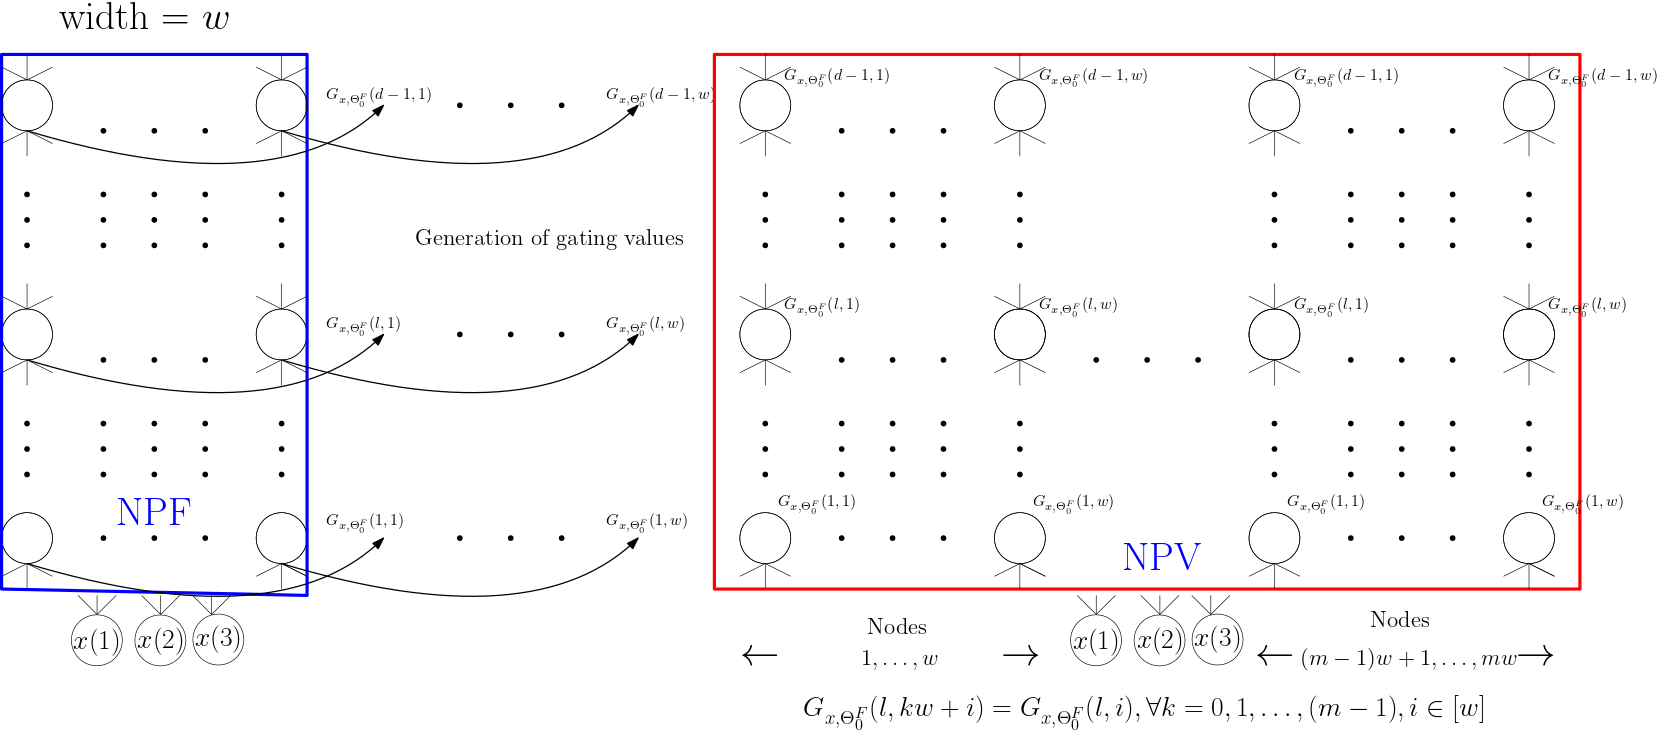
\includegraphics[scale=0.1]{figs/dgn-infty.png}
%}
\caption{DGN${}^{(m)}$ where the value network is of width $mw$ and depth $d$. The gates are derived by padding the gating values obtained from the feature network `$m$' times, i.e., $ G_{x}(kw+i,l)=G_{x}(i,l),\forall k=0,1,\ldots,m-1, i\in[w]$.}
\label{fig:dgnpad}
\end{figure}



\begin{corollary}[Corollary to \Cref{th:main}] Under the same assumptions as in \Cref{th:main} with $\sigma$ replaced by $\sigma_{(m)}=\sigma/\sqrt{m}$, as $m\ra\infty$, \begin{align*}K^{\text{v}}_{\Theta^{\text{DGN}^{(m)}}_0}\ra K^{(d)}_{\text{FNPF}} = d\cdot \sigma_{(m)}^{2(d-1)} H^{(m)}_{\text{FNPF}}= d\cdot \sigma^{2(d-1)} H_{\text{FNPF}}\end{align*}
\end{corollary}
\begin{proof}
Let $\Lambda^{(m)}_{\text{FNPF}}$ and $\tau^{(m)}_{\text{FNPF}}$ be quantities associated with DGN${}^{(m)}$. We know that  $H^{(m)}_{\text{FNFP}}=\Sigma\odot\Lambda^{(m)}_{\text{FNPF}}$. Dropping the subscript FNPF to avoid notational clutter, we have
\begin{align*}
\left(\sigma/\sqrt{m}\right)^{2(d-1)}\Lambda^{(m)}(s,s')&=\sigma^{2(d-1)}\frac{1}{m^{(d-1)}}\Pi_{l=1}^{d-1}\tau^{(m)}(s,s',l)\\
&=\sigma^{2(d-1)}\frac{1}{m^{(d-1)}}\Pi_{l=1}^{d-1}\left(m \tau(s,s',l)\right)\\
&=\sigma^{2(d-1)}\frac{1}{m^{(d-1)}}m^{(d-1)}\Pi_{l=1}^{d-1} \tau(s,s',l)\\
&=\sigma^{2(d-1)}\Pi_{l=1}^{d-1} \tau(s,s',l)\\
&=\sigma^{2(d-1)}\Lambda(s,s')
\end{align*}
\end{proof}


\section{DGN as a Lookup Table: Applying \Cref{th:main} to a pure memorisation task}\label{sec:mem}

In this section, we modify the DGN in \Cref{fig:dgn} into a memorisation network to solve a pure memorisation task. The objective of constructing the memorisation network is to understand the roles of depth and width in \Cref{th:main} in a simplified setting. In this setting, we show increasing depth till a point helps in training and increasing depth beyond it hurts training. 

\begin{definition}[Memorisation Network/Task]
Given a set of values $(y_s)_{s=1}^n\in  \R$, a memorisation network (with weights $\Theta\in\R^{\dnet}$) accepts $s\in[n]$ as its input and produces $\hat{y}_{\Theta}(s)\approx y_s$ as its output. The loss of the memorisation network is defined as $L_{\Theta}=\frac{1}{2}\sum_{s=1}^n (\hat{y}_{\Theta}(s)-y_s)^2$.
\end{definition}
\FloatBarrier
\begin{table}[h]
\centering
\begin{tabular}{| l |  l  |}\hline
Layer&  Memorisation Network\\\hline
Input  &$z_{\Theta}(0)=1$ \\
Pre-Activation & $q_{s,\Theta}(l)=\sum_{j}\Theta(i,j,l)\cdot z_{s,\Theta}(j,l-1)$\\
Hidden & $z_{s,\Theta}(i,l)=q_{s,\Theta}(i,l)\cdot G_{s}(i,l)$ \\
Final  Output & $\hat{y}_{\Theta}(s)=\sum_{j} \Theta(1,j,d) \cdot z_{s,\Theta}(j,d-1)$\\\hline
\end{tabular}
\caption{ Memorisation Network. The input is fixed and is equal to $1$. All the internal variables depend on the index $s$ and the parameter $\Theta$. The gating values $G_s(i,l)$ are external and independent variables.}
\label{tb:dgnmemo}
\end{table}

\textbf{Fixed Random Gating:} The memorisation network is described in \Cref{tb:dgnmemo}. In a memorisation network, the gates are \emph{fixed and random}, i.e., for each index $s\in[n]$, the gating values $G_{s}(i,l),\forall l\in[d-1], i\in[w] $ are sampled from $Ber(\mu), \mu\in(0,1)$ taking values in $\{0,1\}$,  and kept fixed throughout training. The input to the memorisation network is fixed as $1$, and since the gating is fixed and random there is a separate random sub-network to memorise each target $y_s\in\R$. The memorisation network can be used to memorise the targets  $(y_s)_{s=1}^n$ by training it using gradient descent by minimising the squared loss $L_{\Theta}$. In what follows, we let $K_0$ and $H_0$ to be the NTK and NPK of the memorisation network at initialisation.


\textbf{Performance of Memorisation Network:} From \Cref{prop:basic} we know that as $w\ra\infty$, the training error dynamics of the memorisation network follows:
\begin{align}
\dot{e}_t=-K_{0} e_t,
\end{align}
i.e., the spectral properties of $K_0$ (or $H_0$) dictates the rate of convergence of the training error to $0$. In the case of the memorisation network with fixed and random gates, we can calculate $\E{K_0}$ explicitly. 

\textbf{Spectrum of $H_0$:} The input Gram matrix $\Sigma$ is a $n\times n$ matrix with all entries equal to $1$ and its rank is equal to 1, and hence $H_0=\Lambda_0$. We can now calculate the properties of $\Lambda_0$. It is easy to check that $\mathbb{E}_{\mu}\left[\Lambda_0(s,s)\right]=(\mu w)^{(d-1)},\forall s\in[n]$ and $\mathbb{E}_{\mu}\left[\Lambda_0(s,s')\right]=(\mu^2 w)^{(d-1)},\forall s,s'\in[n]$.  For $\sigma=\sqrt{\frac{1}{\mu w}}$, and $\mathbb{E}_{\mu}\left[K_0(s,s)/d\right]=1$, and $\mathbb{E}_{\mu}\left[K_0(s,s')/d\right]=\mu^{(d-1)}$. 
\begin{figure}
\centering
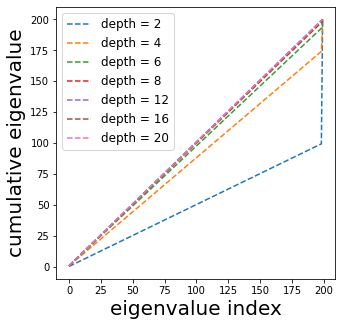
\includegraphics[scale=0.3]{figs/dgn-fra-ecdf-ideal-small.png}
\caption{Ideal spectrum of $\E{K_0}/d$ for a memorisation network for $n=200$.}
\label{fig:ideal-spectrum}
\end{figure}


\textbf{Why increasing depth till a point helps ?} 
We have:
%\comment{
\begin{align}\label{eq:mat}
\frac{\E{K_0}}{d}=\left[\begin{matrix}
1 &\mu^{d-1} &\ldots &\mu^{d-1} &\ldots\\ 
\ldots &1 &\ldots &\mu^{d-1} &\ldots\\ 
\ldots &\mu^{d-1} &\ldots &1 &\ldots \\
\ldots &\mu^{d-1} &\ldots &\mu^{d-1} &1\\ 
\end{matrix}\right]
\end{align}
%}
i.e., all the diagonal entries are $1$ and non-diagonal entries are $\mu^{d-1}$. Now, let $\rho_i\geq 0,i \in [n]$ be the eigenvalues of $\frac{\E{K_0}}{d}$, and let $\rho_{\max}$ and $\rho_{\min}$ be the largest and smallest eigenvalues.  One can easily show that $\rho_{\max}=1+(n-1)\mu^{d-1}$ and corresponds to the eigenvector with all entries as $1$, and $\rho_{\min}=(1-\mu^{d-1})$ repeats $(n-1)$ times,  which corresponds to eigenvectors given by $[0, 0, \ldots, \underbrace{1, -1}_{\text{$i$ and $i+1$}}, 0,0,\ldots, 0]^\top \in \R^n$ for $i=1,\ldots,n-1$. Note that as $d\ra\infty$, $\rho_{\max},\rho_{\min}\ra 1$.

\textbf{Why increasing depth beyond a point hurts?} 
As the depth increases the variance of the entries $K_0(s,s')$ deviates from its expected value $\E{K_0(s,s')}$. Thus the structure of the Gram matrix degrades from \eqref{eq:mat}, leading to smaller eigenvalues.
%\FloatBarrier
\begin{figure}
\resizebox{\textwidth}{!}{
\begin{tabular}{cccc}
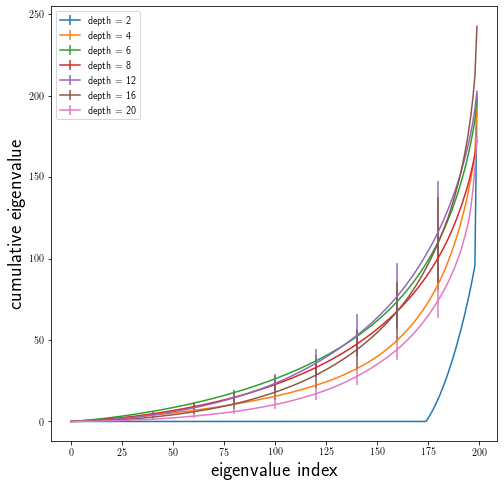
\includegraphics[scale=0.5]{figs/dgn-fra-ecdfbyd-w25.png}
&
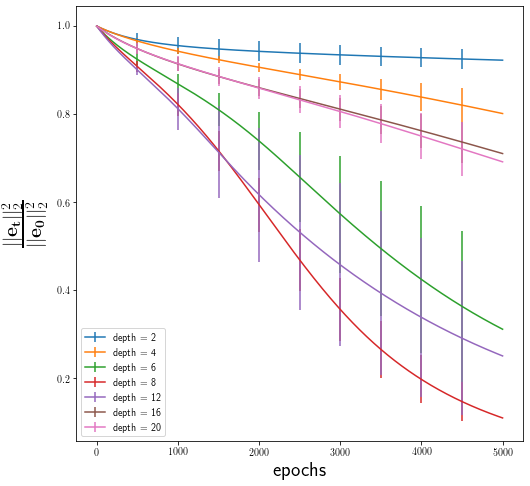
\includegraphics[scale=0.5]{figs/dgn-fra-conv-w25.png}
&
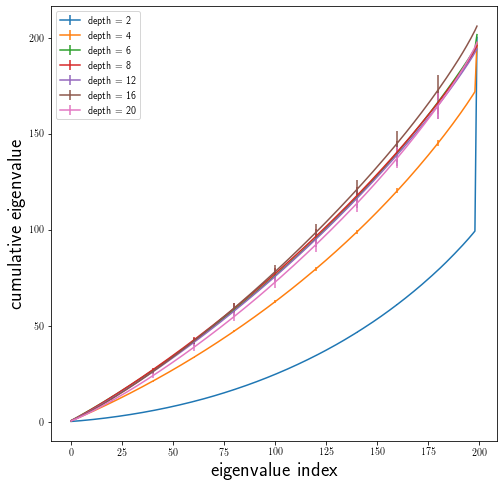
\includegraphics[scale=0.5]{figs/dgn-fra-ecdfbyd-w500.png}
&
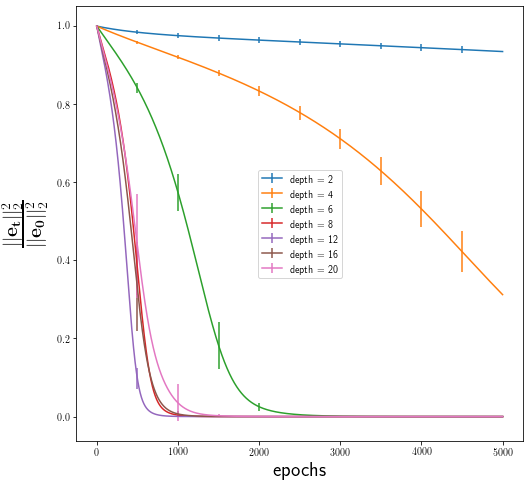
\includegraphics[scale=0.5]{figs/dgn-fra-conv-w500.png}
\end{tabular}
}
\caption{Shows the plots for the memorisation network with $\mu=\frac{1}{2}$ and $\sigma=\sqrt{\frac{2}{w}}$. The number of points to be memorised is $n=200$. The left most plot shows the e.c.d.f for $w=25$ and the second plot from the left shows the error dynamics during training for $w=25$. The second plot from the right shows the e.c.d.f for $w=500$ and the right most plot shows the error dynamics during training for $w=500$. All plots are averaged over $10$ runs.}
\label{fig:dgn-frg-gram-ecdf}
\end{figure}

\subsection{Experiment}
We set $n=200$, and $y_s\sim\text{Uniform}[-1,1]$. We look at the cumulative eigenvalue (e.c.d.f) obtained by first sorting the eigenvalues in ascending order then looking at their cumulative sum. The ideal behaviour (\Cref{fig:ideal-spectrum}) as predicted from theory is that for indices $k\in[n-1]$, the e.c.d.f should increase at a linear rate, i.e., the cumulative sum of the first $k$ indices is equal to $k(1-\mu^{d-1})$, and the difference between the last two indices is $1+(n-1)\mu^{d-1}$. In \Cref{fig:dgn-frg-gram-ecdf}, we plot the actual e.c.d.f for various depths $d=2,4,6,8,12,16,20$ and $w=25,500$ (first and third plots from the left in \Cref{fig:dgn-frg-gram-ecdf}). 

\textbf{Roles of depth and width:} In order to compare how the rate of convergence varies with the depth, we set the step-size $\alpha=\frac{0.1}{\rho_{\max}}$, $w=100$. We use the vanilla SGD-optimiser. Note the$ \frac{1}{\rho_{\max}}$ in the stepsize, ensures that the uniformity of maximum eigenvalue across all the instances, and the convergence should be limited by the smaller eigenvalues. We also look at the convergence rate of the ratio $\frac{\norm{e_t}^2_2}{\norm{e_0}^2_2}$. We notice that for $w=25$, increasing depth till $d=8$ improves the convergence, however increasing beyond $d=8$ worsens the convergence rate. For $w=500$, increasing the depth till $d=12$ improves convergence, and $d=16,20$ are worse than $d=12$.  %This matches with the depth phenomena observed in practical DNNs and also matches our theory.
\end{appendix}

\end{document}
